%-----------------------------------------------------------------------
% Beginning of chap3.tex
%-----------------------------------------------------------------------
%
%%%%%%%%%%%%%%%%%%%%%%%%%%%%%%%%%%%%%%%%%%%%%%%%%%%%%%%%%%%%%%%%%%%%%%%%

\chapter[RESULTS]{Results}
\vspace{-12pt}
\section{Ecosystem Metabolism}

Across all sites, median GPP ranged from 0.12 to 0.77 \unit{\goxy}, while median ER ranged -0.84 to -10.85 \unit{\goxy}. ER exceeded GPP across all sites, resulting in median NEP ranging from -0.35 to -10.41 \unit{\goxy} (Table \ref{tab:GPP-ER}). All sites were heterotrophic, i.e, where ER exceeds GPP, with very few (1-4) autotrophic days. Across all sites, day to day variability in GPP (CV 1.16 \%) was low whereas ER (CV -1.18 \%) exhibited slightly more daily variation than GPP (Figure~\ref{fig:GPPvER}). There was a subtle increase in GPP across the precipitation gradient, with the exception of GC where median GPP was low (0.25 \unit{\goxy}), falling in line with the most arid sites (Figure~\ref{fig:GPPBox}). 

Unlike GPP, there was no discernible pattern in ER (Figure~\ref{fig:ERBox}) nor in NEP (Figure~\ref{fig:NEPBox}) from semi-arid to mesic study sites. ER varies across the precipitation gradient, but ER at WMC  was 3-13 fold greater than the other sites (Table~\ref{Tab:GPPandER}). At PDC, I was only able to estimate metabolism for 279 days out of the nearly 2 years of data because the stream was completely dry or was disconnected pools during 2020-2021 (Table~\ref{Tab:GPPandER}).


Between SFC, AR, and PLC there appeared to be slight spring and summer increases in GPP and ER across the precipitation gradient in 2020, there is not the same pattern in 2017. GPP increased later into the summer as precipitation increased along the gradient (Figure~\ref{Fig:MetabStacked}).

\begin{figure}[htb]
\begin{center}
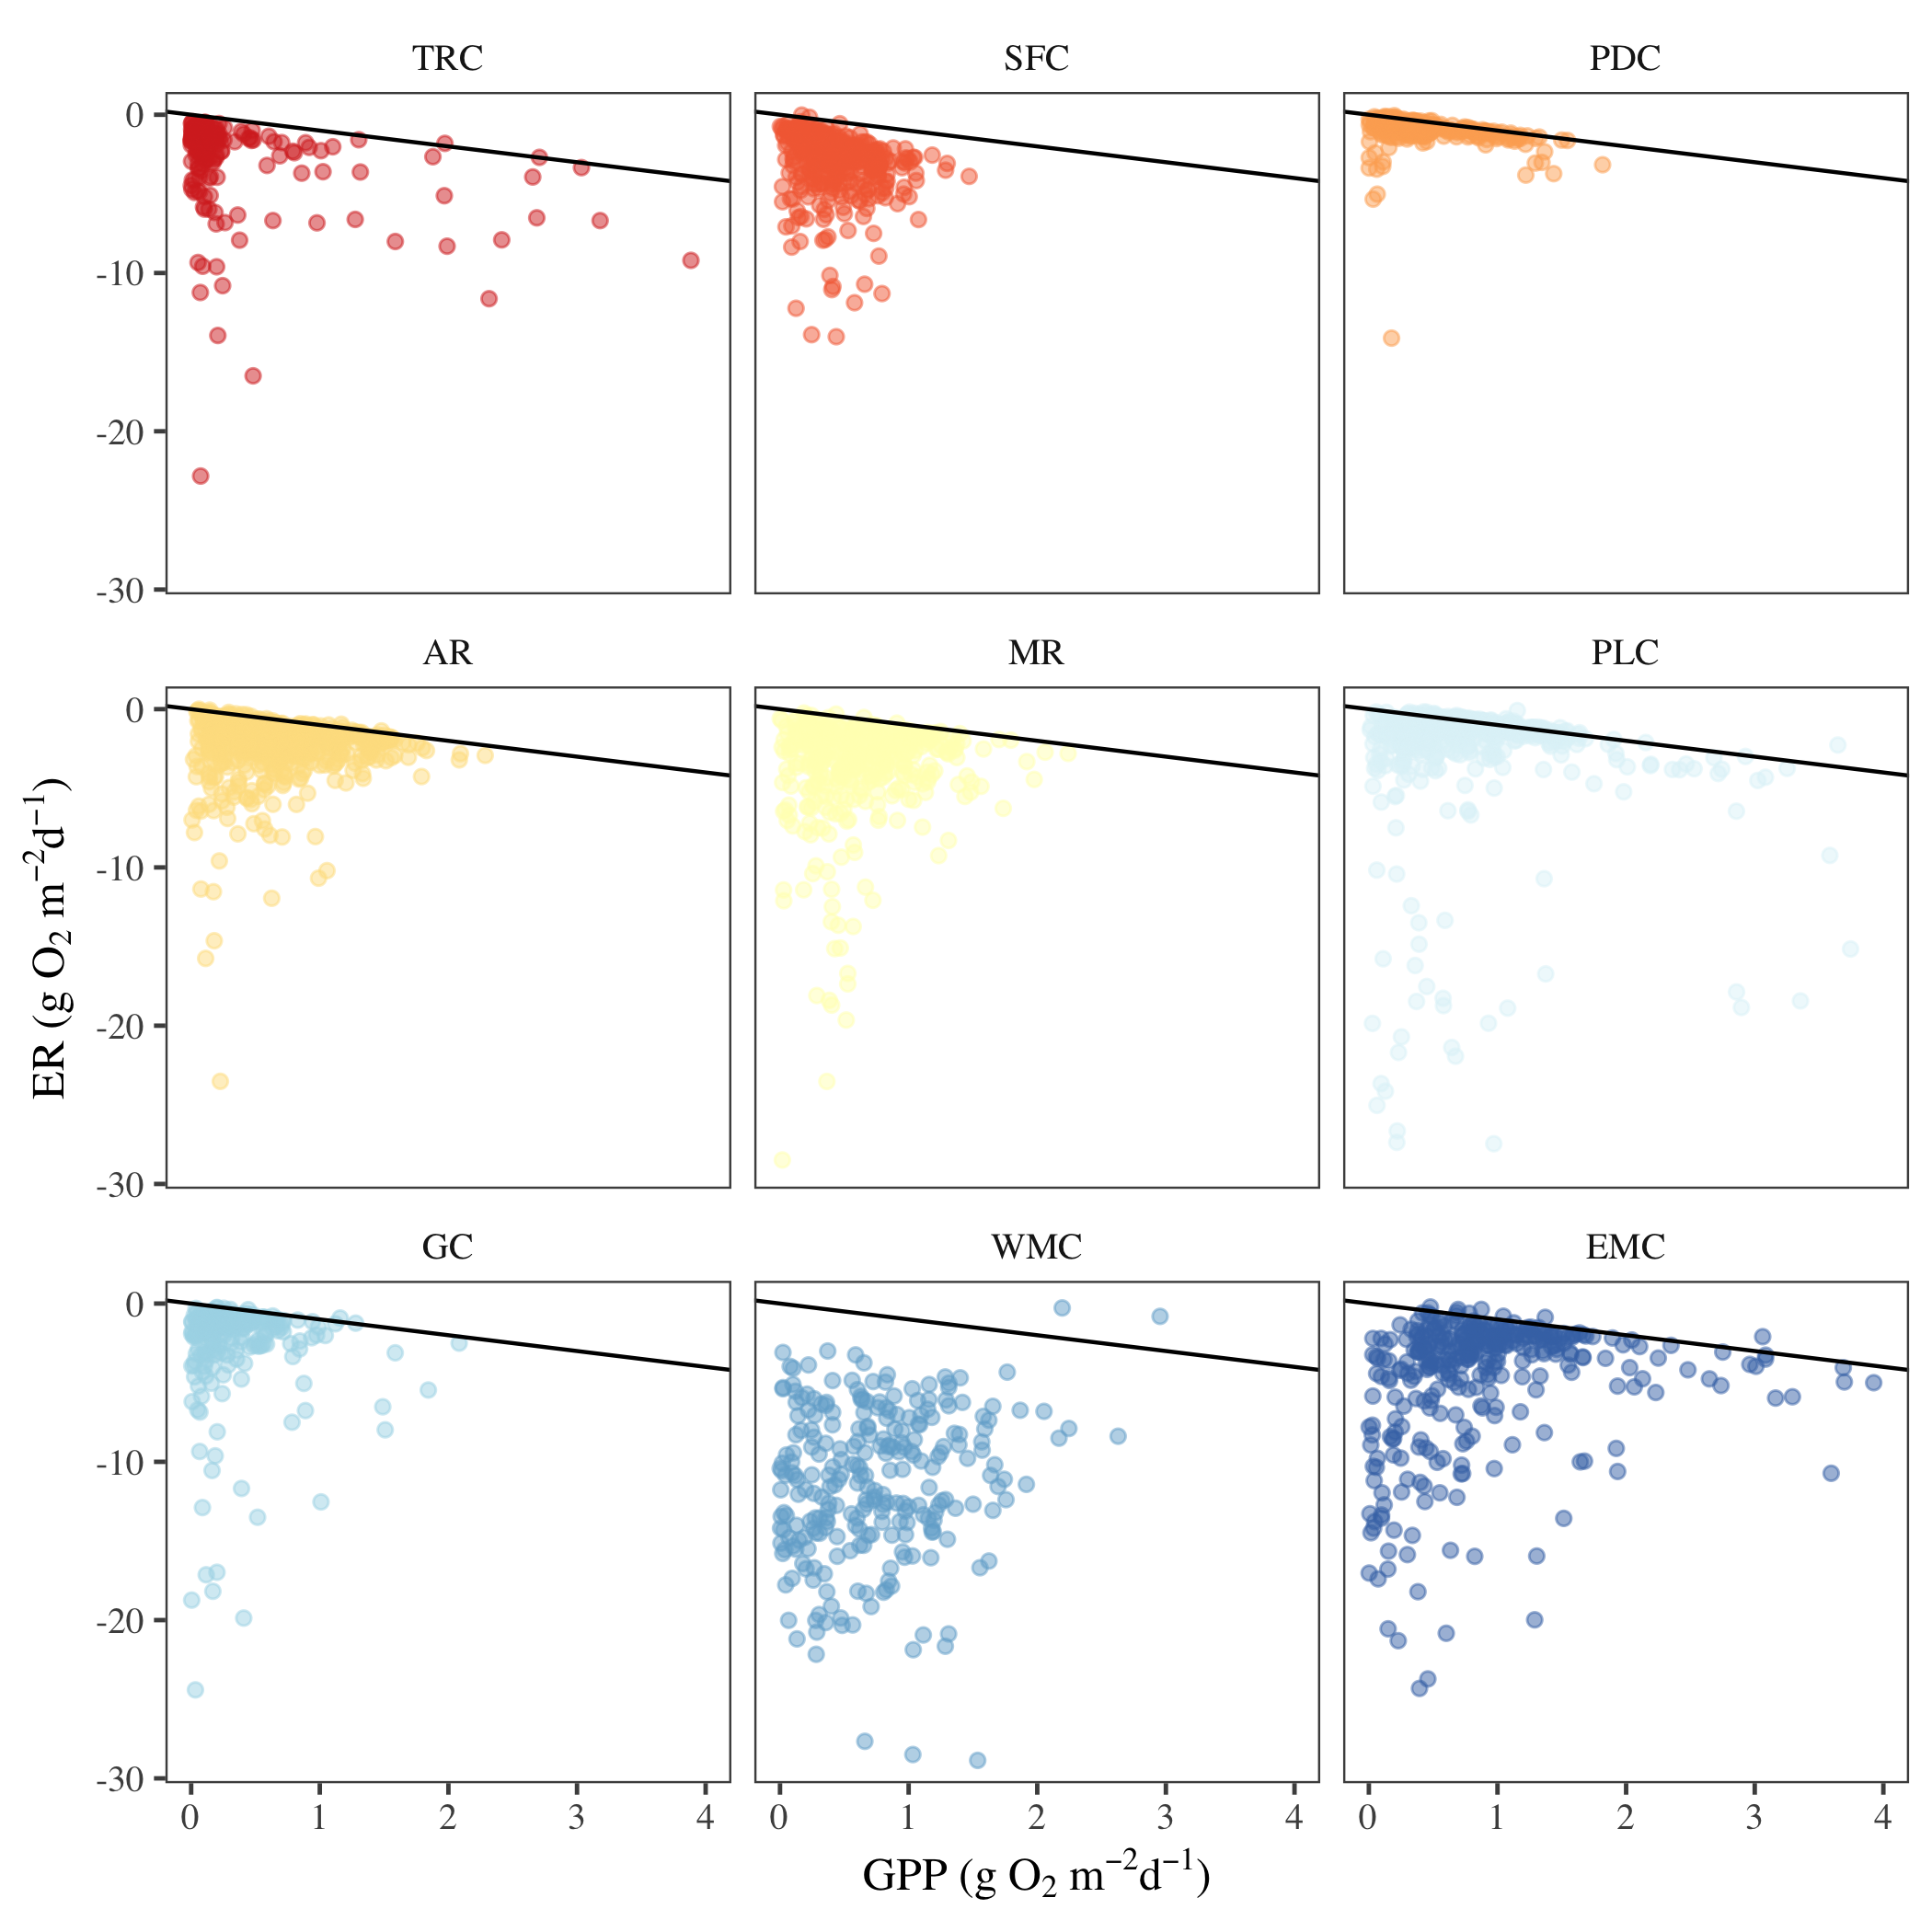
\includegraphics[scale=0.2]{Figs/GPPvER.png}
\caption[Gross Primary Production and Ecosystem Respiration]{\textit{Gross Primary Production and Ecosystem Respiration}. Sites are arranged from arid to mesic left to right and top to bottom (red to blue). Points above the 1:1 line indicate days of autotrophy where gross primary production (GPP) exceeds ecosystem respiration (ER), and points below are heterotrophic days were ER exceeds GPP. Across all sites, ER was more variable than GPP with very few autotrophic days (e.g. 2 days at WMC and 1 day at PLC and EMC).}
\small 
\label{fig:GPPvER}
\end{center}
\end{figure}

\begin{figure}[htb]
\begin{center}
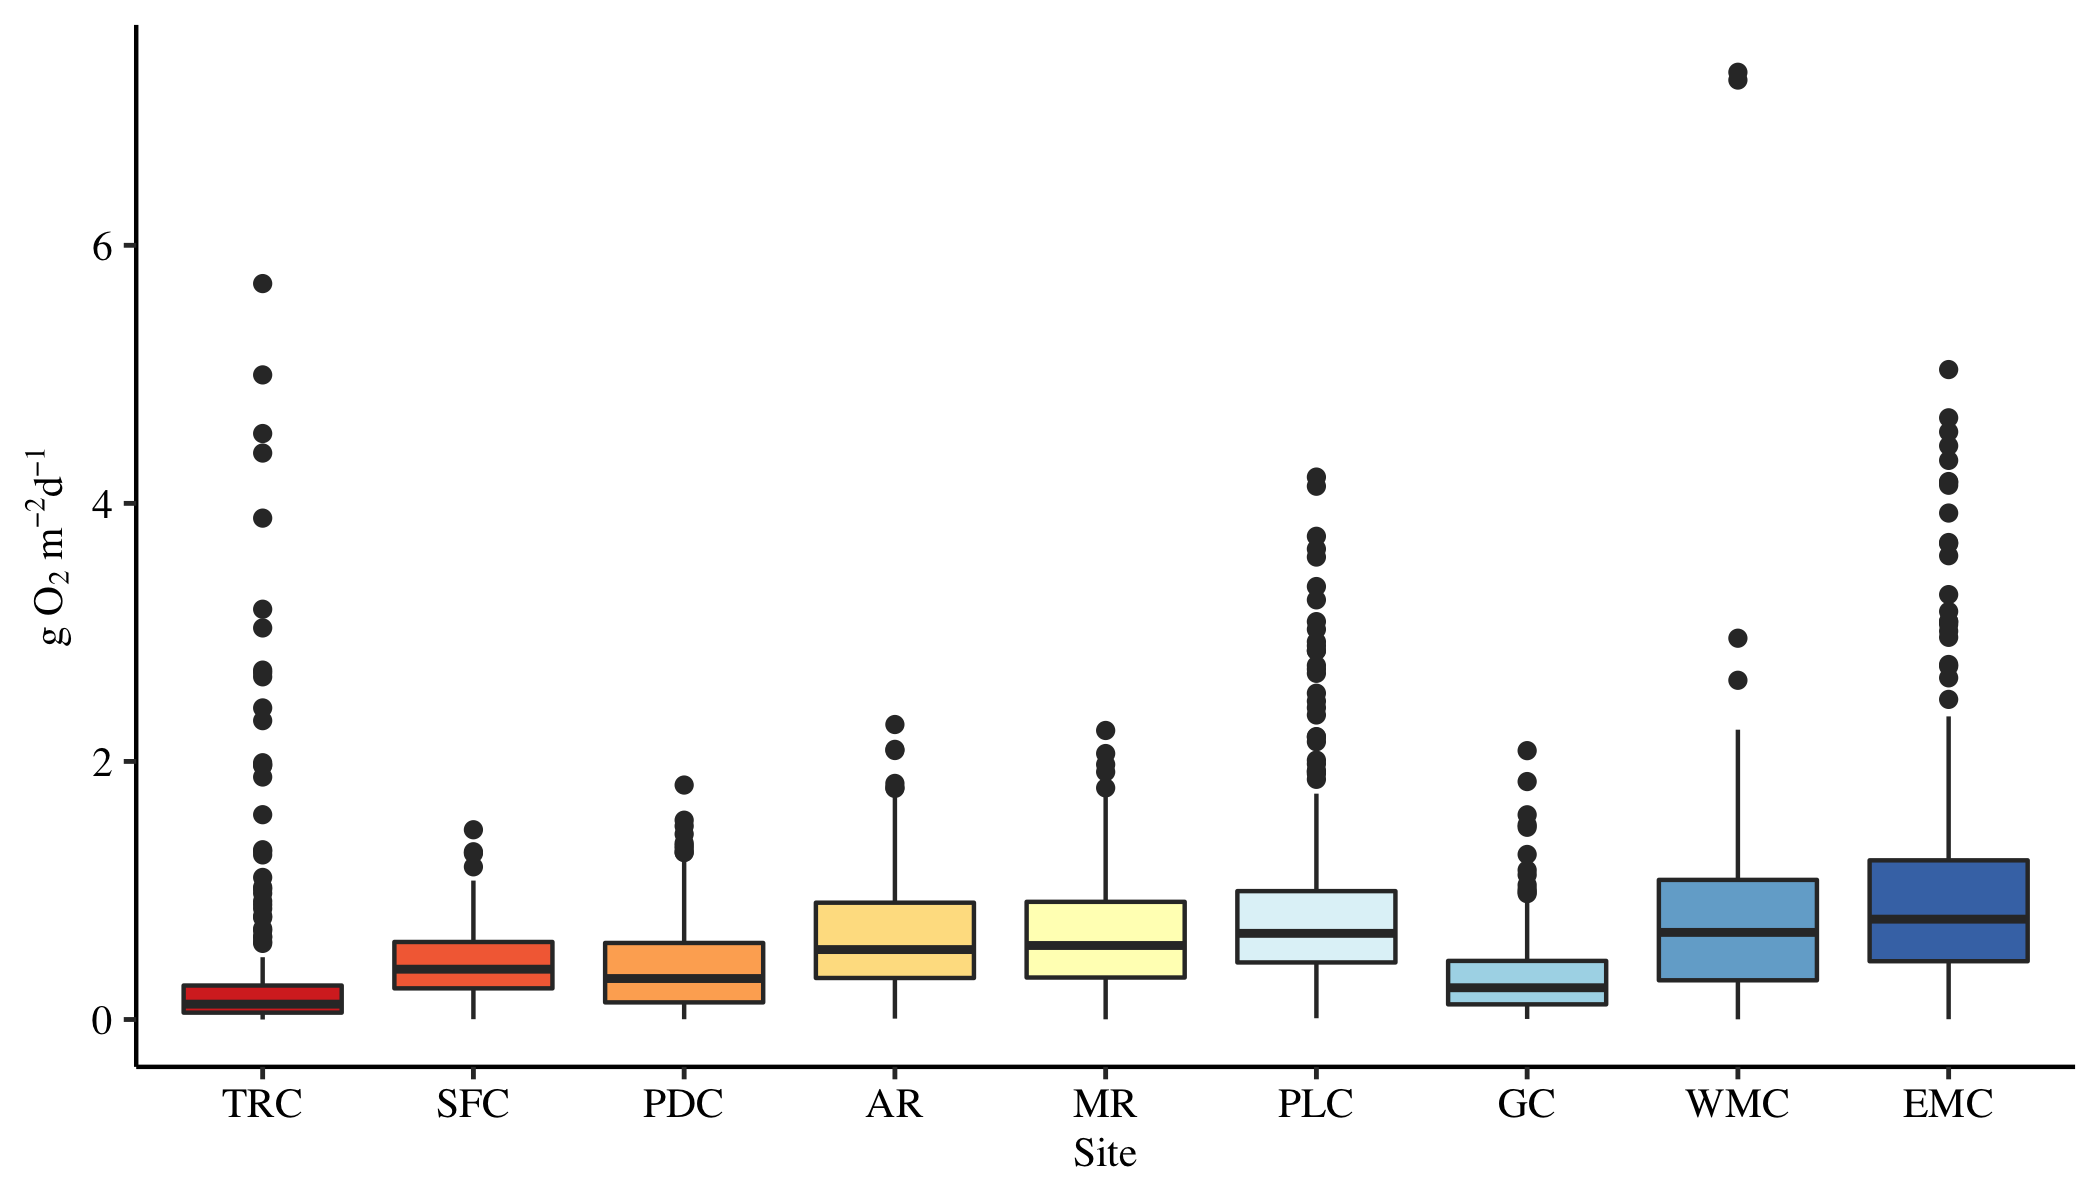
\includegraphics[scale=0.2]{Figs/GPPBox.png}
\caption[Gross Primary Production]{\textit{Gross Primary Production}. There was a subtle increase in GPP across the precipitation gradient (sites are arranged arid to mesic, left to right), with the exception of GC, falling in line with the most arid sites. The boxes are the middle 50 quartile (25 to 75), the line is the median, the tails are 1.5X interquartile range, and any points falling outside of the line are considered outliers.}
\label{fig:GPPBox}
\end{center}
\end{figure}

\begin{figure}[htb]
\begin{center}
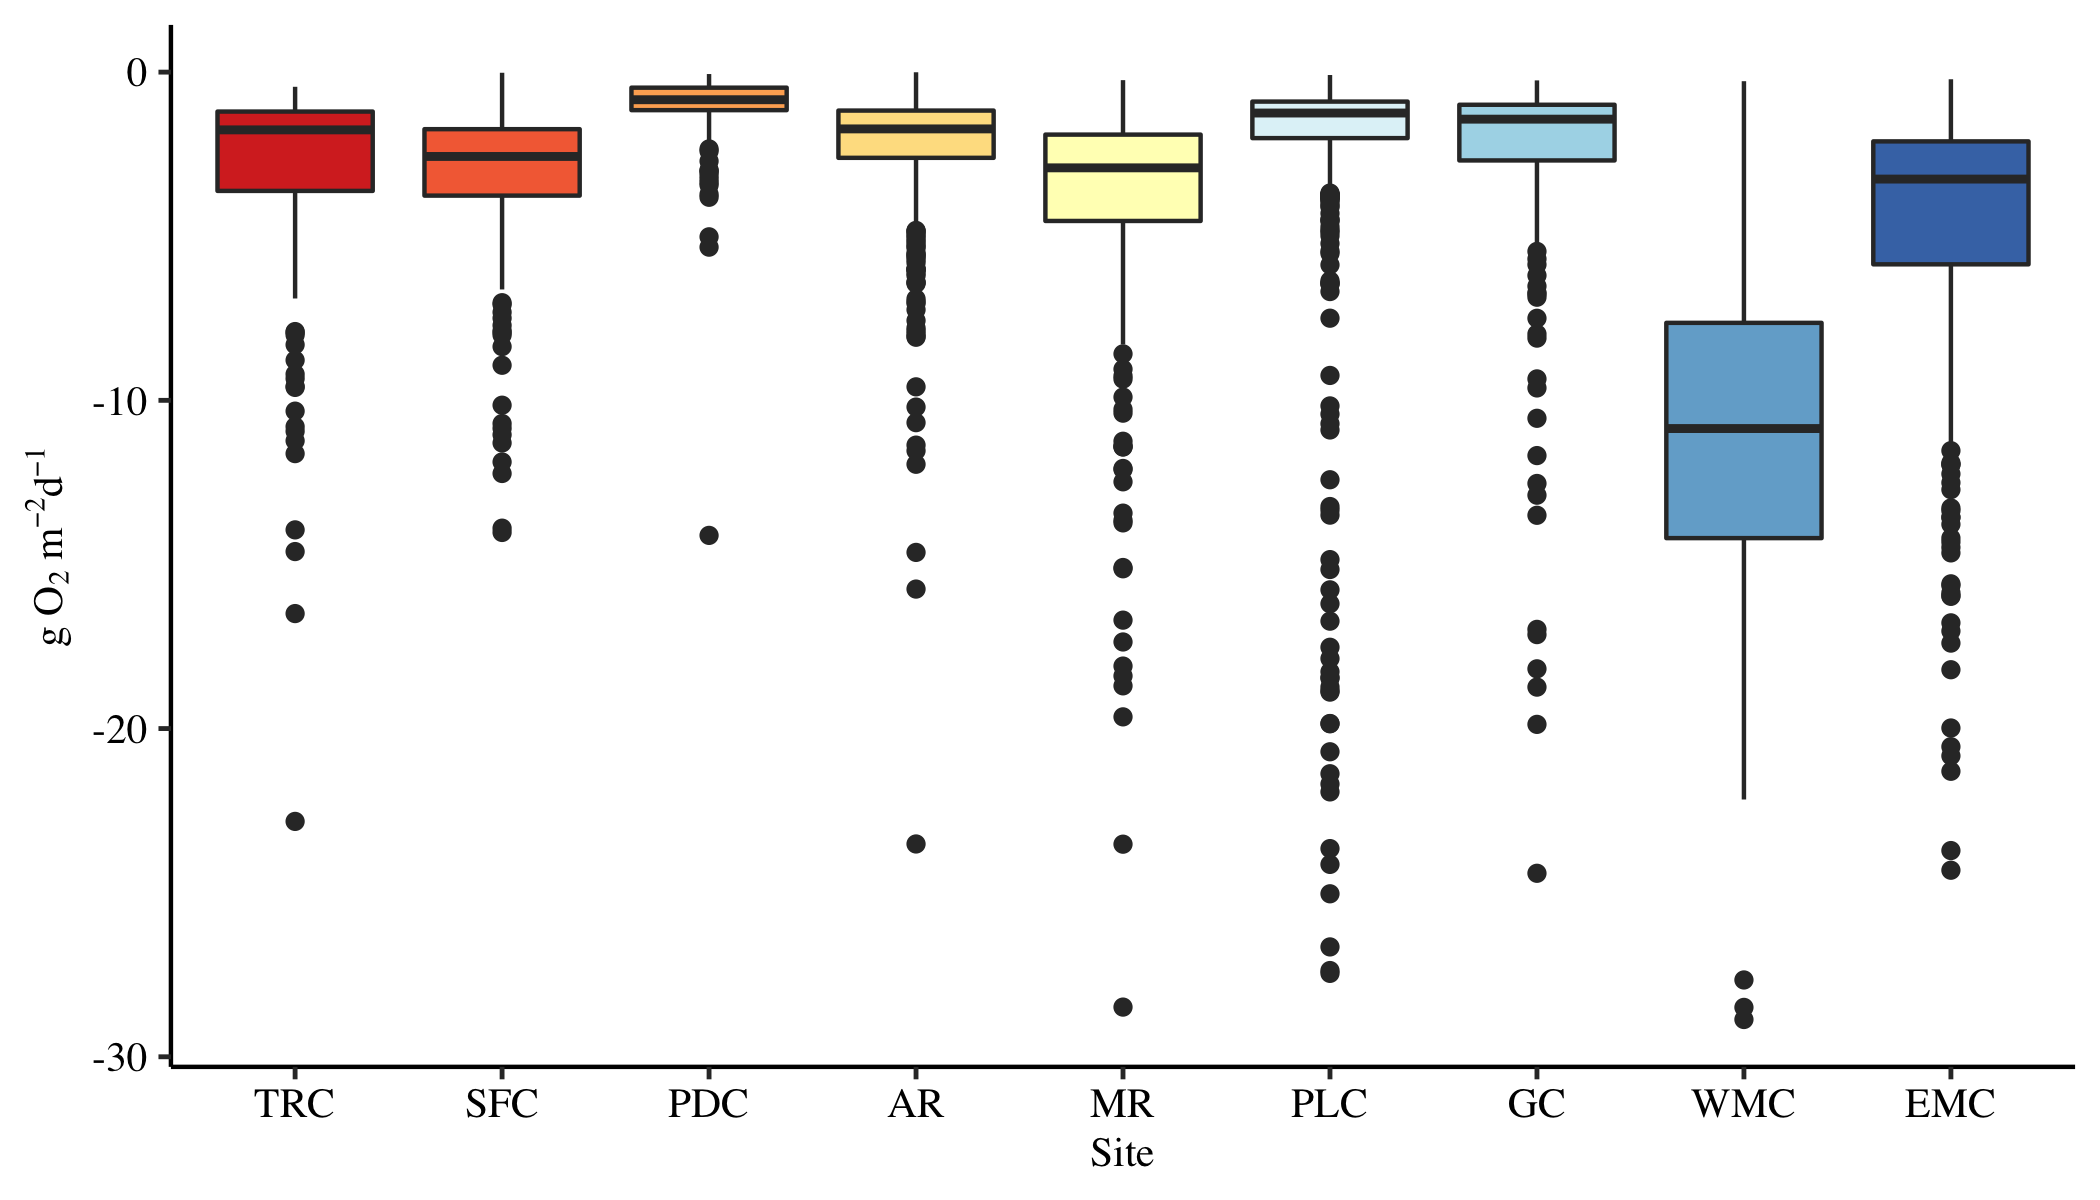
\includegraphics[scale=0.2]{Figs/ERBox.png}
\caption[Ecosystem Respiration]{\textit{Ecosystem Respiration}. There appears to be no discernible pattern in ecosystem respiration (ER) along the precipitation gradient (sites are arranged arid to mesic, left to right). The boxes are the middle 50 quartile (25 to 75), the line is the median, the tails are 1.5X interquartile range, and any points falling outside of the line are considered outliers.}
\label{fig:ERBox}
\end{center}
\end{figure}

\begin{figure}[htb]
\begin{center}
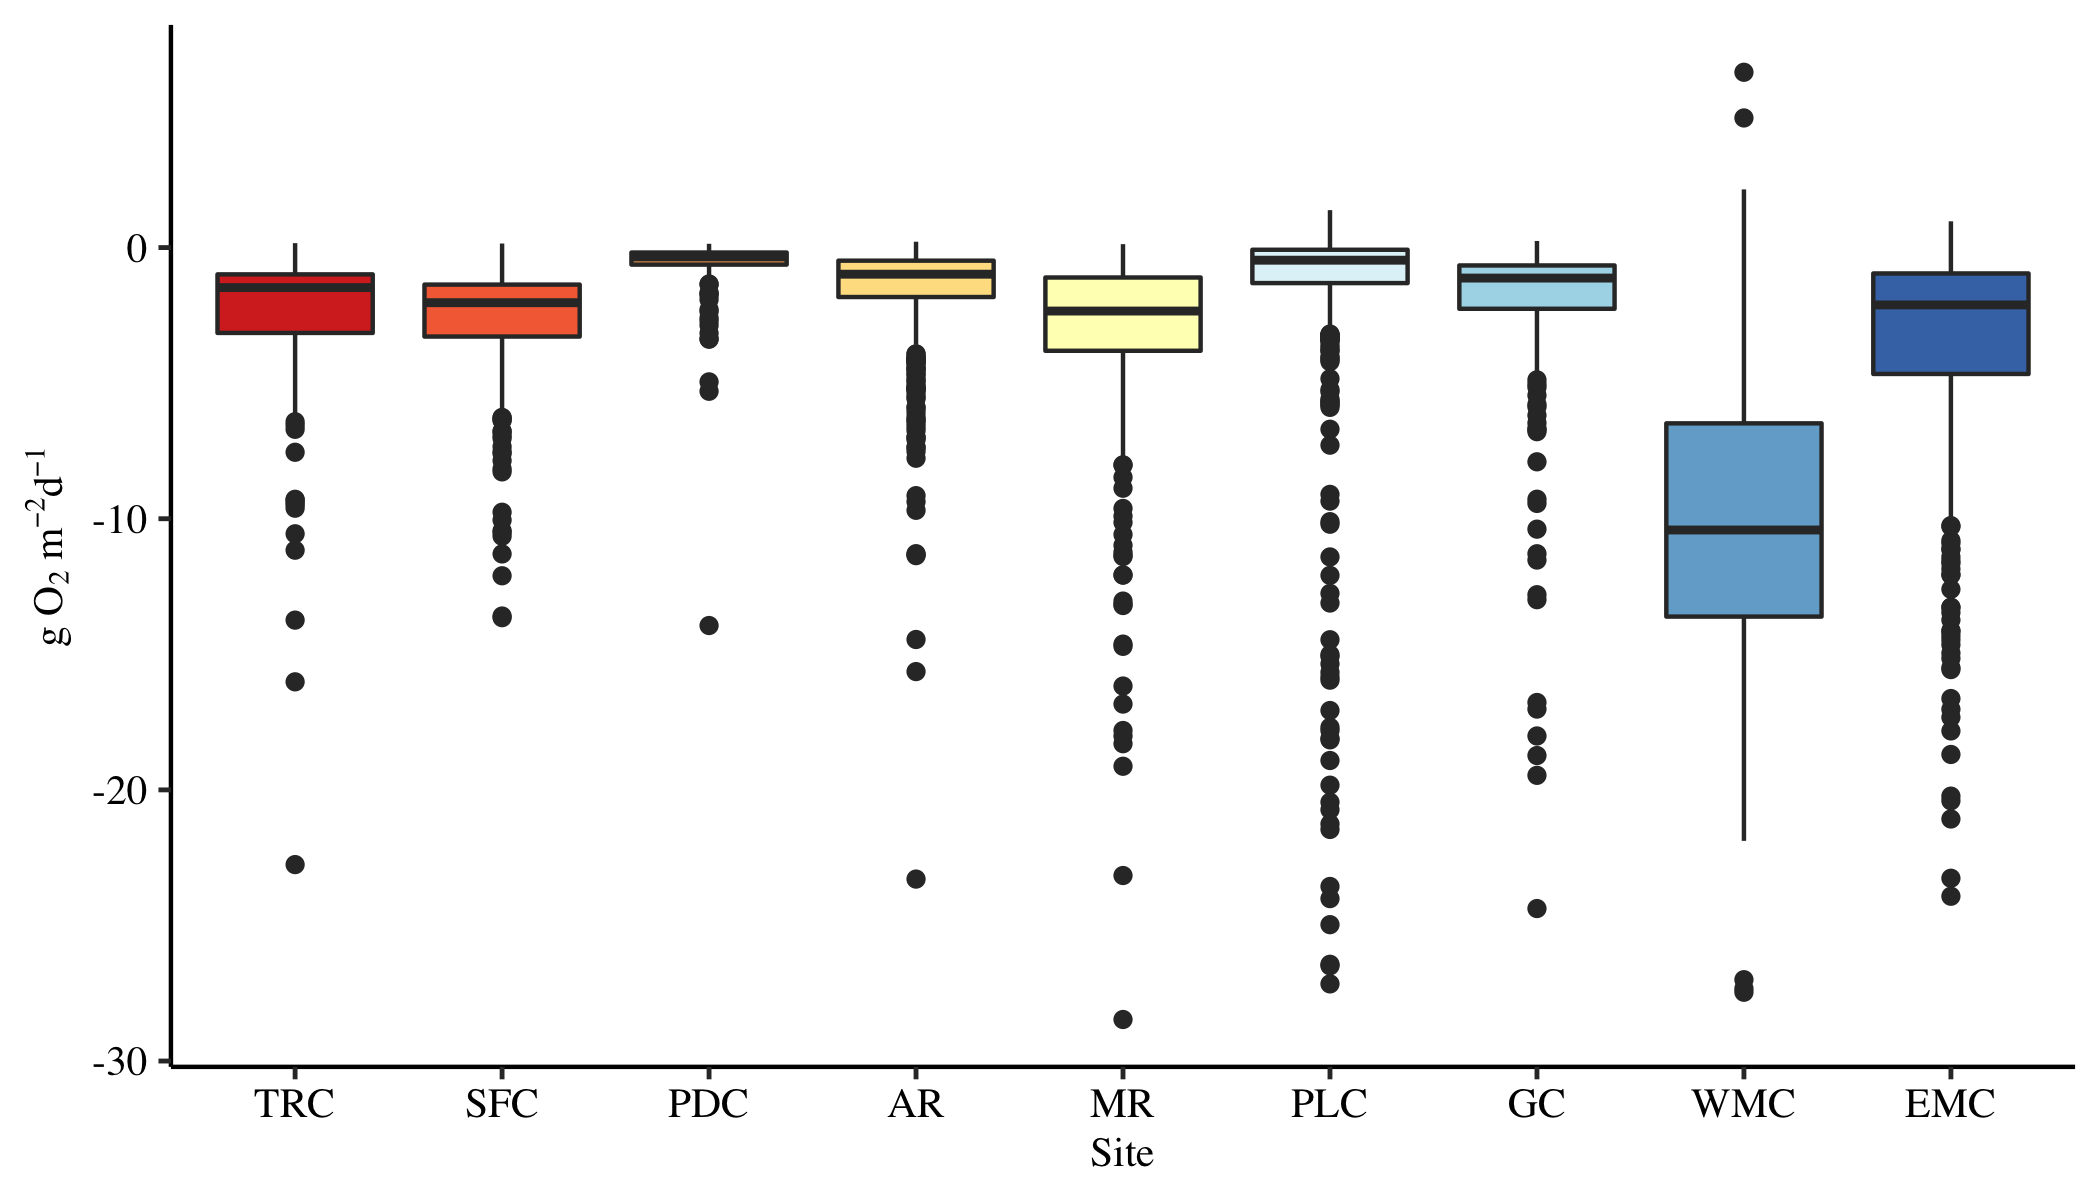
\includegraphics[scale=0.2]{Figs/NEPBox.png}
\caption[Net Ecosystem Production]{\textit{Net Ecosystem Production}. There appears to be no discernible pattern in net ecosystem production (NEP) along the precipitation gradient (sites are arranged arid to mesic, left to right). The boxes are the middle 50 quartile (25 to 75), the line is the median, the tails are 1.5X interquartile range, and any points falling outside of the line are considered outliers.}
\label{fig:NEPBox}
\end{center}
\end{figure}

\begin{landscape}
\begin{figure}[htb]
\begin{center}
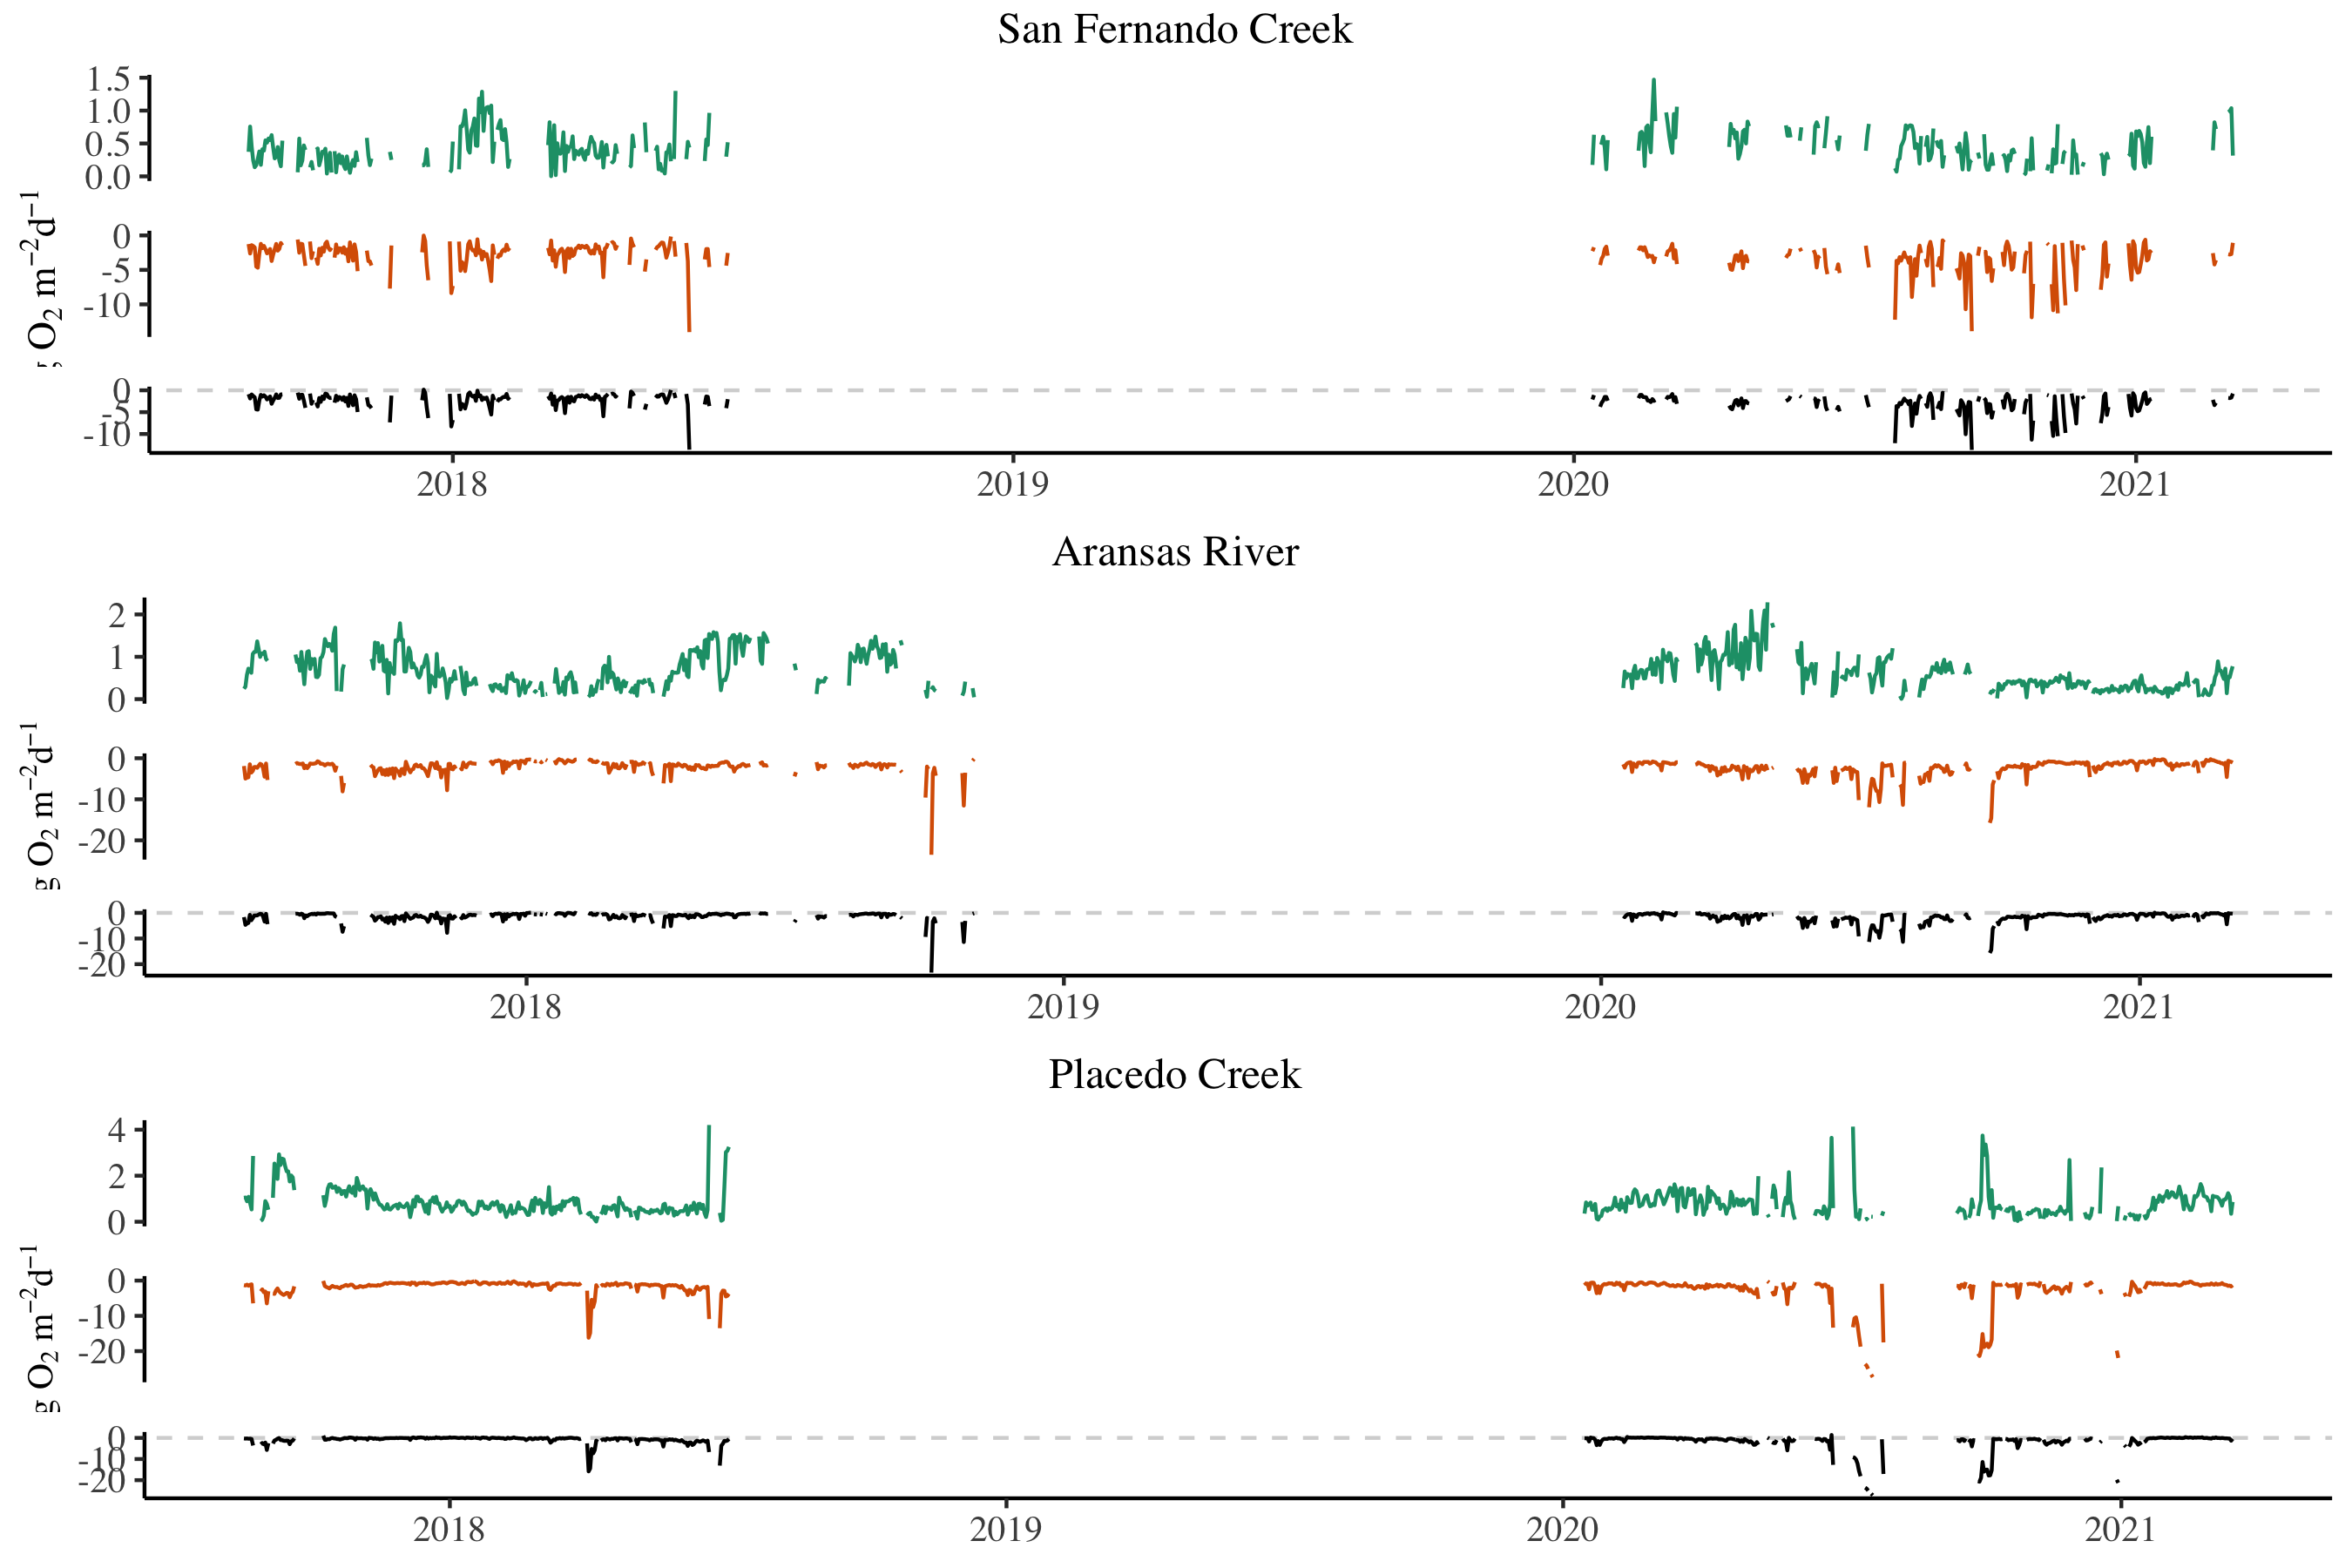
\includegraphics[scale=0.2]{Figs/MetabStacked.png}
\caption[Ecosystem Metabolism for Three Sites]{\textit{Ecosystem Metabolism for Three Sites}. Sites are arranged arid to mesic top down. Daily gross primary production (GPP, green lines) does not appear to have a distinct seasonal pattern  from 2017-2018. In comparison, during 2020, GPP appeared to vary seasonally across the sites shown here. GPP appears to increase later into the summer along the precipitation gradient, from arid to mesic. Ecosystem respiration (ER, orange lines) has the same pattern but appears to lag behind GPP. Daily net ecosystem production (NEP, black line) mirrors ER.}
\label{Fig:MetabStacked}
\end{center}
\end{figure}
\end{landscape}

\begin{landscape}
\begin{table}[htb]
\caption[Metabolism Summary]{\textit{Metabolism Summary}}\label{Tab:GPPandER}
\begin{center}
\begin{tabular}{cccccccc}
\hline\noalign{\smallskip}
Site & Usable Days & \makecell {Median GPP \\(\unit{\goxy})} & GPP 95\% CI & \makecell {Median ER \\(\unit{\goxy})} & ER 95\% CI & \makecell {Median NEP \\(\unit{\goxy})} & NEP 95\% CI\\\hline
TRC & 185 & 0.12 & 0.09-0.14 & -1.80 & -1.16 - -2.10 & -1.50 &-1.30- -1.70 \\ \
SFC & 365 & 0.39 & 0.37-0.43 & -2.60 & -2.40- -2.80 & -2.00 & -1.90- -2.20\\ 
AR & 686 & 0.54 & 0.49-0.58 & -1.70 & -1.60- -1.80 & -0.98 & -0.89- -1.10\\ 
PDC & 279 & 0.32 & 0.27-0.37 & -0.84 & -0.73- -0.93 & -0.35 & -0.30- -0.42\\ 
MR & 382 & 0.57 & 0.53-0.63 & -2.90 & --2.70- -3.10 & -2.30 & -2.00- -2.60\\ 
PLC & 609 & 0.67 & 0.63-0.71 & -1.20 & -1.20 - -1.30 & -0.46 & -0.39- -0.53\\ 
GC & 233 & 0.25 & 0.21-0.28 & -1.40 & -1.30 - -1.60 & -1.10 &  -0.97- -1.30\\ 
WMC & 263 & 0.67 & 0.62-0.79 & -11.00 & -10.00 - -12.00 & -10.00 & -9.40- -11.00\\ 
EMC & 352 & 0.78 & 0.72-0.83 & -3.30 & -3.00 - -3.60 & -2.10 & -1.80- -2.50 \\ 
\noalign{\smallskip}\hline
\end{tabular}
\end{center}
\small \textit{Note}: Number of days where I was able to estimate ecosystem metabolism, median gross primary production estimates, median ecosystem respiration estimates, and median net ecosystem production of the nine sites. CI, confidence intervals. Sites are arranged from arid to mesic top down.
\label{tab:GPP-ER}
\end{table}
\end{landscape}


\section{DOC and Nutrients}

Across all sites, average DOC ranged from 5.3 to 12.5 \unit{\mg\per\L} (Figure~\ref{Fig:DOC}). Along the precipitation gradient from semi-arid SFC to semi-mesic GC, average DOC increased (from 6.4 to 9.3 \unit{\mg\per\L}); however, average DOC concentrations at EMC, where land use is predominantly agriculture, were 5.5 \unit{\mg\per\L}, and did not follow the pattern of increasing DOC concentrations along the precipitation gradient (Figure~\ref{Fig:DOC}). Similarly, DOC concentrations at TRC, the driest site with the most non-agricultural vegetation, was the highest along the gradient (12.5 \unit{\mg\per\L}) (Table \ref{tab: Nutrients}).

Unlike DOC concentrations, there were no discernible patterns in nutrients across the precipitation gradient. Two of the sites (SFC and AR) had high levels of NO$_3$-N and PO$_4$-P, 20-185x higher for NO$_3$-N and 10-35x higher for PO$_4$-P (Figure \ref{Fig:Nitrate}~and~\ref{Fig:SPR}). Both of these sites receive waste water treatment plant effluent.

\begin{figure}[htb]
\begin{center}
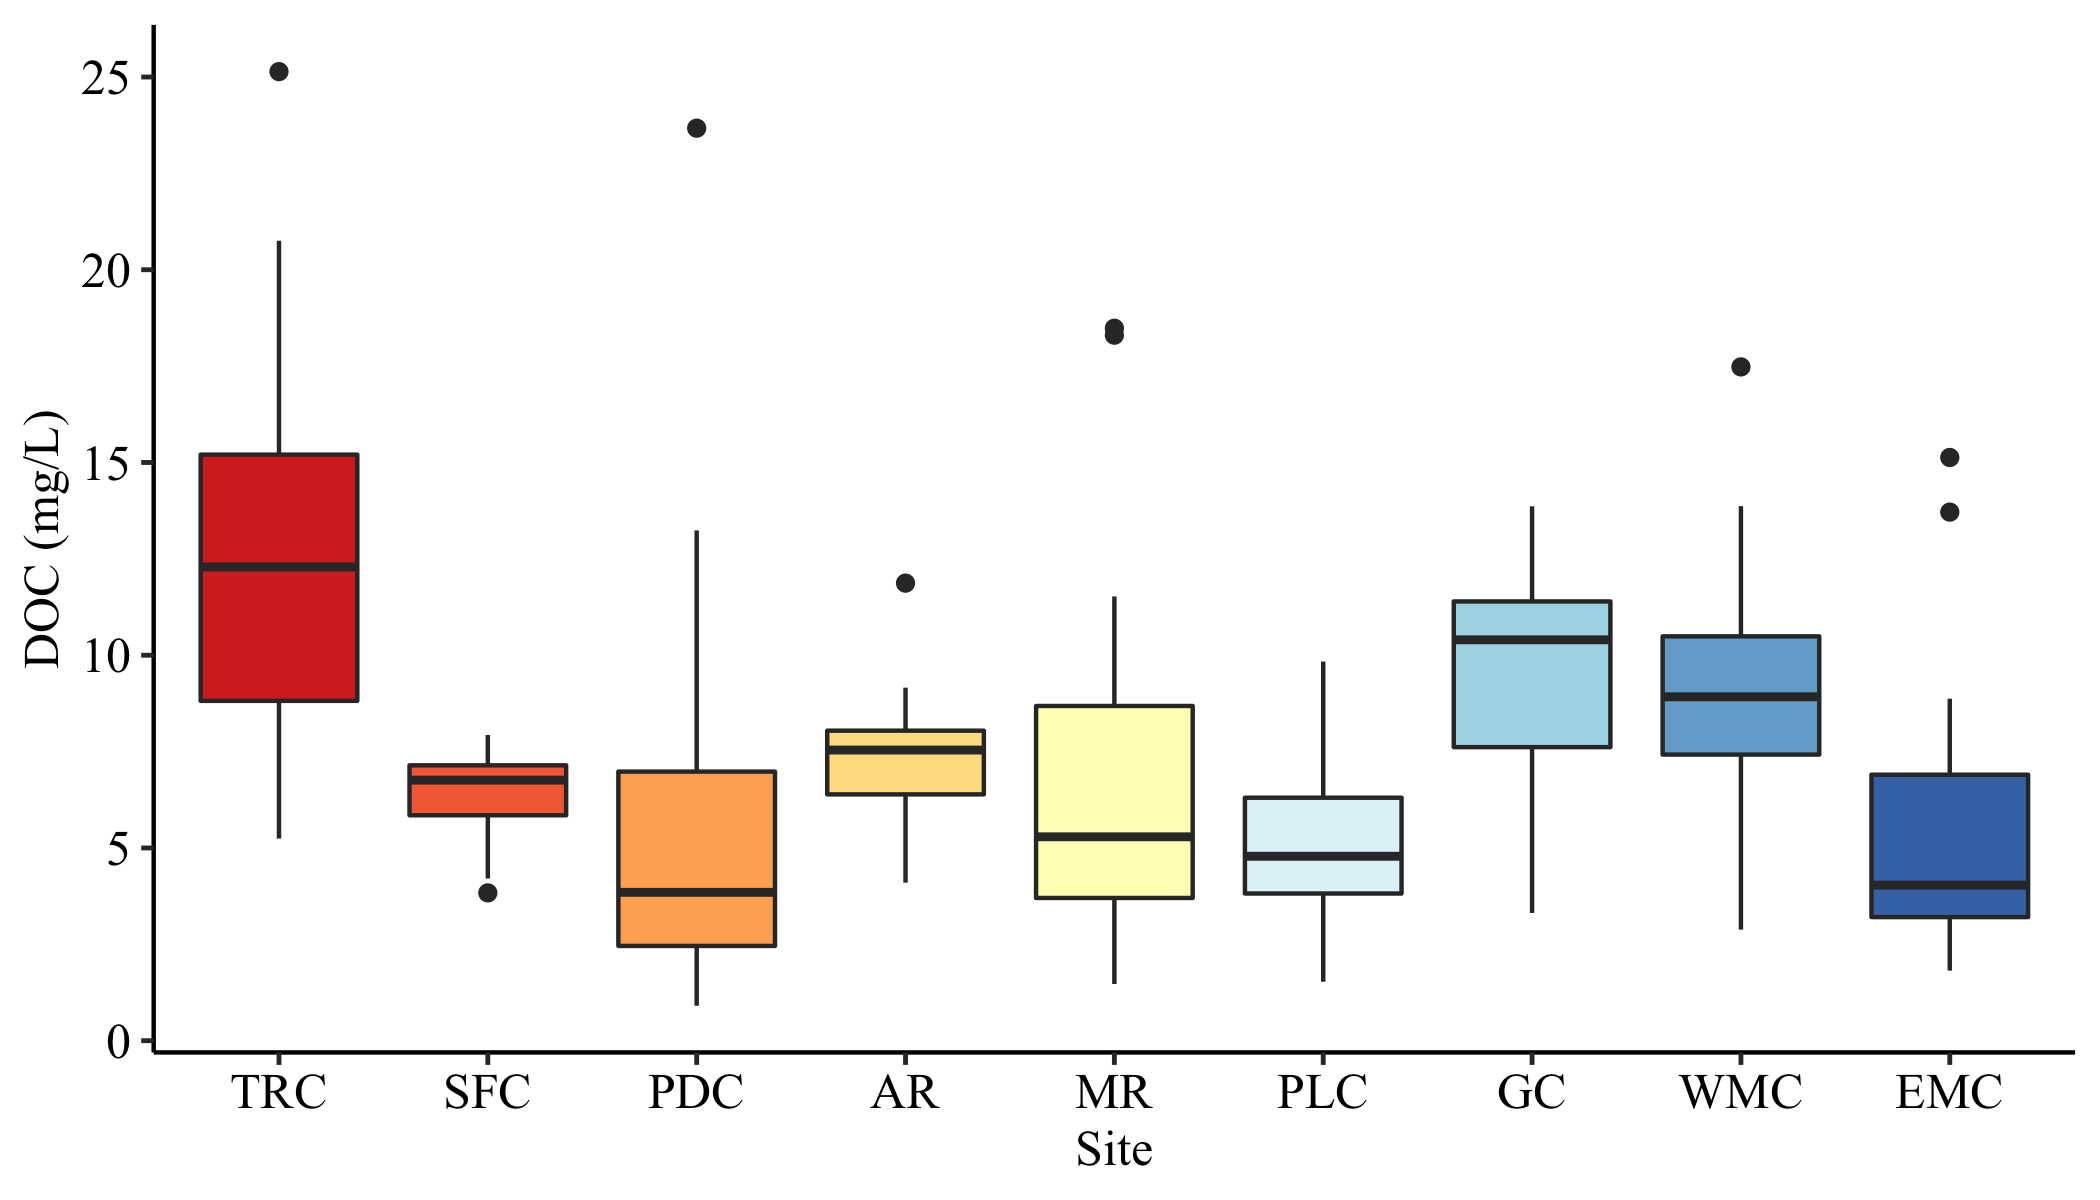
\includegraphics[scale=0.2]{Figs/DOC.png}
\caption[Dissolved Organic Carbon]{\textit{Dissolved Organic Carbon}. Sites are arranged arid to mesic left to right. Dissolved organic carbon appears to increase as precipitation increases (left to right). However, TRC and EMC do not follow this pattern. The boxes are the middle 50 quartile (25 to 75), the line is the median, the tails are 1.5X interquartile range, and any points falling outside of the line are considered outliers.
}\label{Fig:DOC}
\end{center}
\end{figure}

\begin{figure}[htb]
\begin{center}
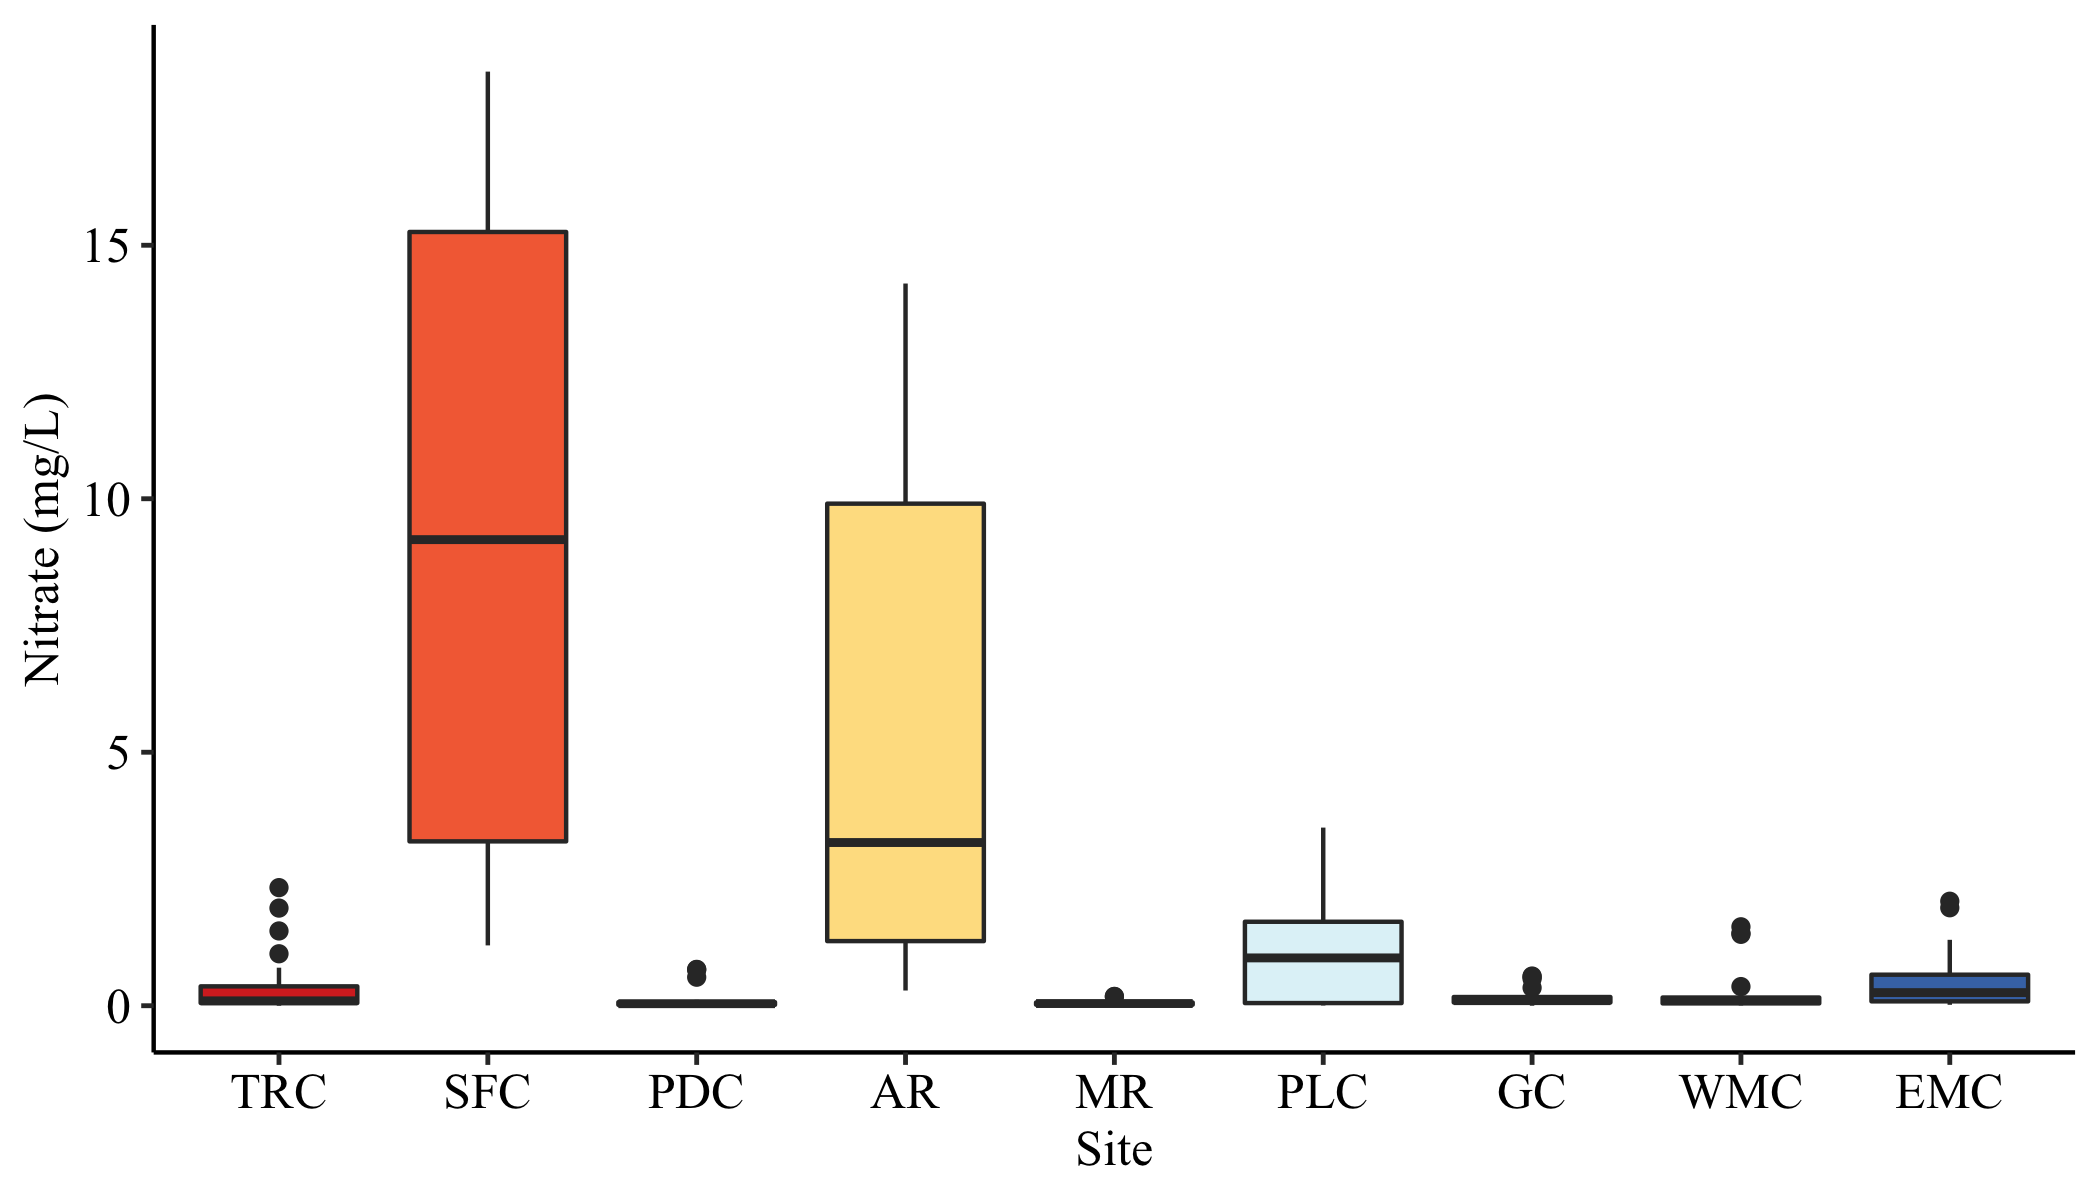
\includegraphics[scale=0.2]{Figs/NitrBox.png}
\caption[Nitrate]{\textit{Nitrate}. There does not appear to be a trend in nitrate across the precipitation gradient (Sites are arranged arid to mesic, left to right), however, SFC and AR had concentrations 20-185x higher than other study sites. The boxes are the middle 50 quartile (25 to 75), the line is the median, the tails are 1.5X interquartile range, and any points falling outside of the line are considered outliers.}
\label{Fig:Nitrate}
\end{center}
\end{figure}

\begin{figure}[htb]
\begin{center}
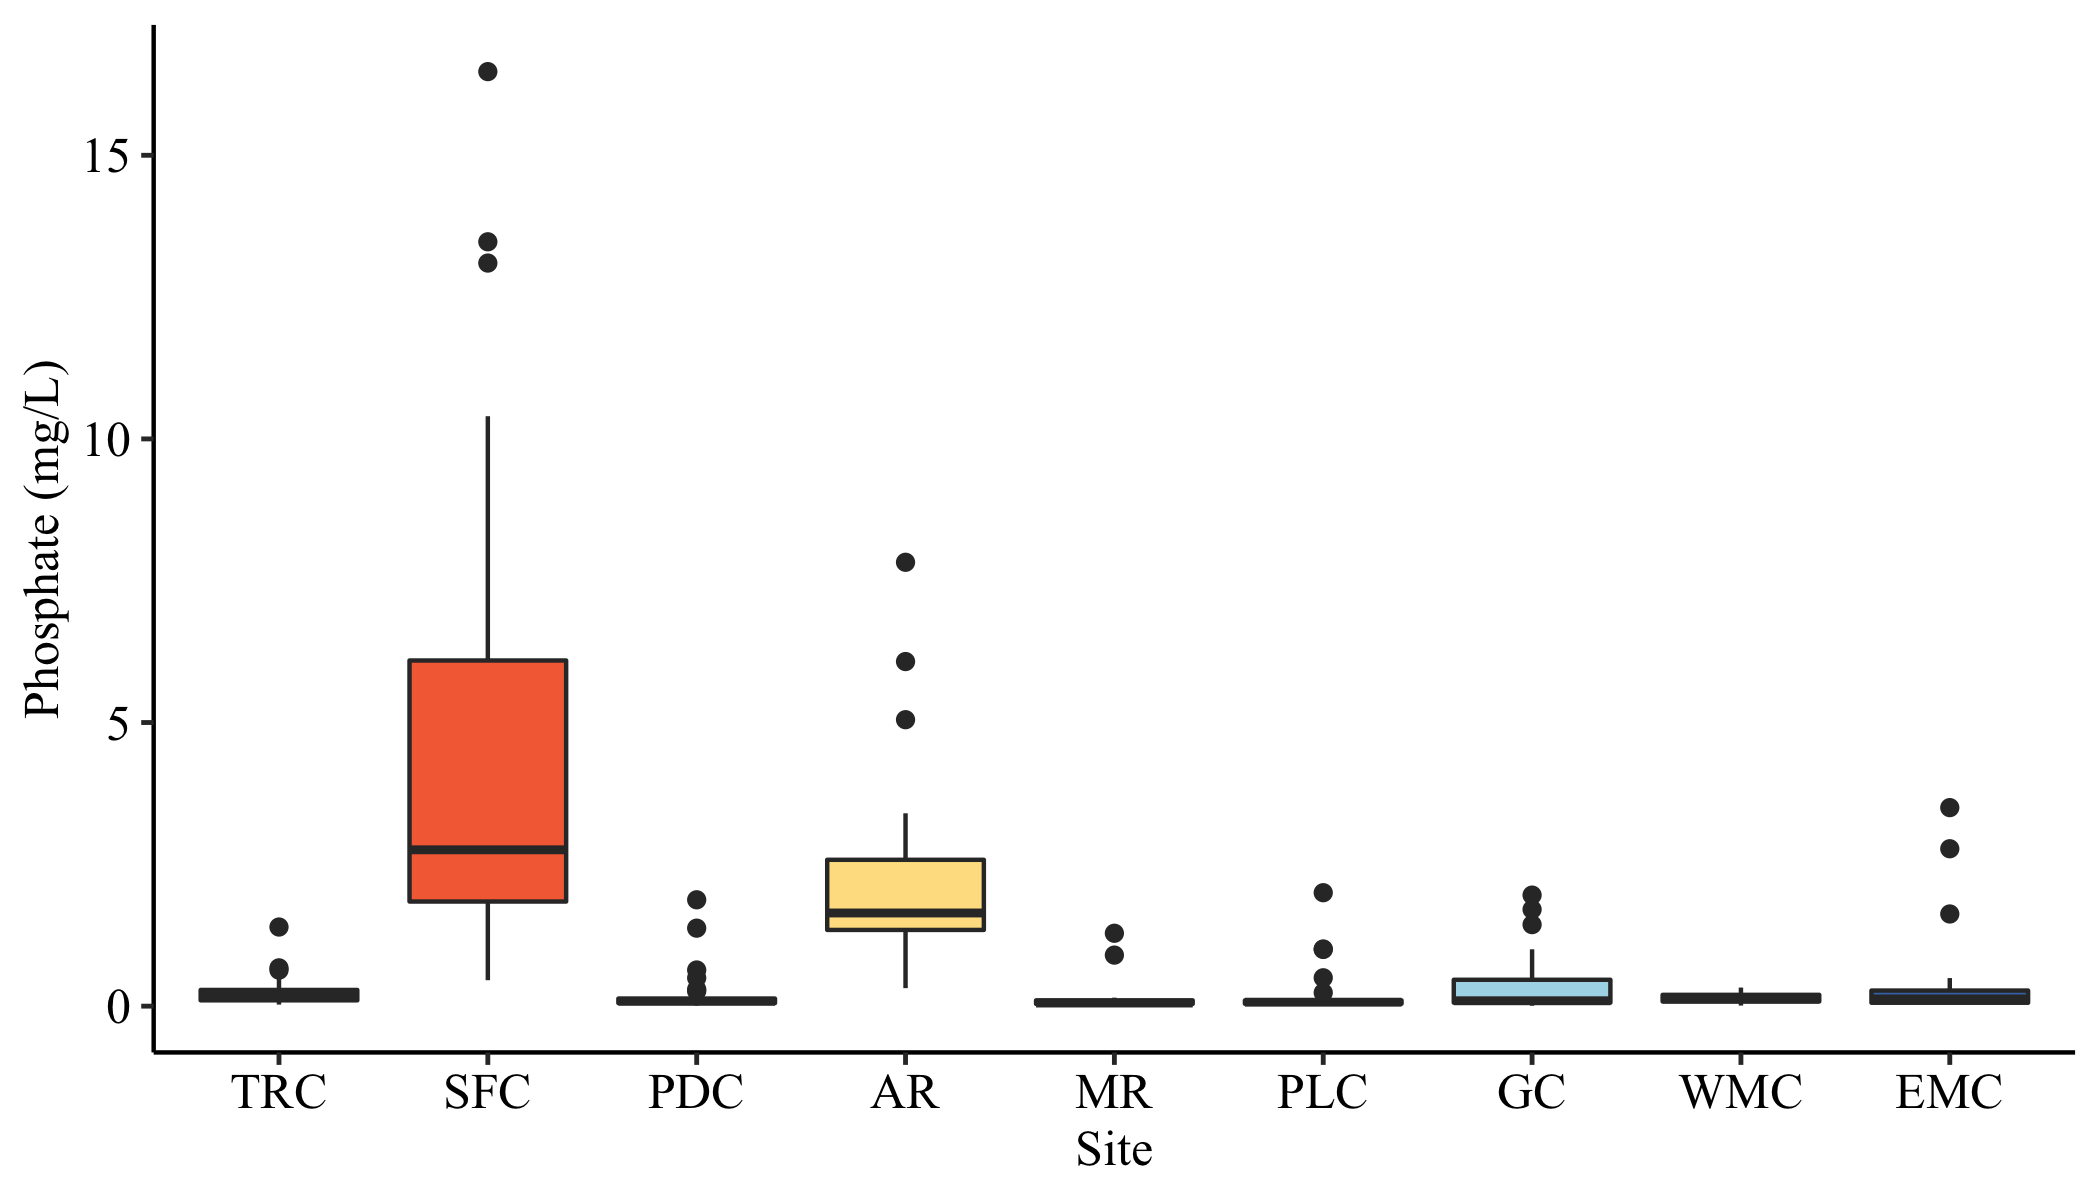
\includegraphics[scale=0.2]{Figs/OrthoPBox.png}
\caption[Soluble Reactive Phosphorous]{\textit{Soluble Reactive Phosphorous}. There does not appear to be a trend in soluble reactive phosphorous across the precipitation gradient (Sites are arranged arid to mesic, left to right), however, SFC and AR had concentrations 10-35x higher than other study sites. The boxes are the middle 50 quartile (25 to 75), the line is the median, the tails are 1.5X interquartile range, and any points falling outside of the line are considered outliers.}
\label{Fig:SPR}
\end{center}
\end{figure}

\begin{table}[htb]
\caption[DOC and Nutrient Concentrations]{\textit{DOC and Nutrient Concentrations}}
\begin{center}
\begin{tabular}
[c]{ccccc}\hline
Site & \makecell {DOC $\pm$ SD\\(\unit{\mg\per\L})} & \makecell {NH$_4$-N $\pm$ SD\\(\unit{\mg\per\L})} & \makecell {NO$_3$-N $\pm$ SD\\(\unit{\mg\per\L})} & \makecell {PO$_4$-P $\pm$ SD\\(\unit{\mg\per\L})}\\\hline
TRC & 12.5 $\pm$ 4.8 & 0.22 $\pm$ 0.16 & 0.39 $\pm$ 0.61 & 0.27 $\pm$ 0.28\\
SFC & 6.4 $\pm$ 1.16 & 0.18 $\pm$ 0.01 & 9.25 $\pm$ 6.0 & 4.60 $\pm$ 4.40\\
AR & 7.2 $\pm$ 1.80 &0.16 $\pm$ 0.14 & 5.1 $\pm$ 4.50 & 2.22 $\pm$ 1.70\\
PDC & 5.8 $\pm$ 5.40 & 0.14 $\pm$ 0.01 & 0.11 $\pm$ 0.20 & 0.23 $\pm$ 0.42\\
MR & 6.9 $\pm$ 4.70 & 0.13 $\pm$ 0.10 & 0.05 $\pm$ 0.05 & 0.13 $\pm$ 0.30\\
PLC	 & 5.3 $\pm$ 2.40 & 0.13 $\pm$ 0.05 & 1.06 $\pm$ 1.21 & 0.23 $\pm$ 0.44\\
GC & 9.3 $\pm$ 3.15 & 0.18 $\pm$ 0.22 & 0.16 $\pm$ 0.16 & 0.39 $\pm$ 0.56\\
WMC & 9.1 $\pm$ 3.20 & 0.13 $\pm$ 0.063 & 0.26 $\pm$ 0.45 & 0.14 $\pm$ 0.08\\
EMC & 5.5 $\pm$ 3.55 & 0.13 $\pm$ 0.07 & 0.45 $\pm$ 0.54 & 0.42 $\pm$ 0.83\\\hline
\end{tabular}
\end{center}
\textit{Note}: Average concentrations of dissolved organic carbon (DOC), ammonium (NH$_4$-N), nitrate (NO$_3$-N), and phosphate (PO$_4$-P) across the precipitation gradient (sites are arranged arid to mesic, top down). San Fernando Creek and Aransas River both receive water from waste water treatment plants. SD, standard deviation.
\label{tab: Nutrients}
\end{table}

\section{Discharge}

Across the precipitation and land use gradients, average discharged ranged from \qtyrange{.03}{3.00}{\cubic\m\per\second}, with WMC having the highest discharge, and PDC the flashiest (Table~\ref{tab:Q}). Across the gradients, discharge greatly varied between sites and had quick responses to storm events (Figure \ref{Fig:Q}).

\begin{table}
\caption[Summary of Site Discharge]{\textit{Summary of Site Discharge}}
\begin{center}
\begin{tabular}[c]{ccccc}
\hline
Site & \makecell{Mean Discharge\\(\unit{\cubic\m\per\s})} & \makecell{Median Discharge\\(\unit{\cubic\m\per\s})} & \makecell{CV\\(\%)}\\
\hline
TRC & 0.03 & 0.00 & 447.32\\
SFC & 0.19 & 0.03 & 1586.92\\
PDC & 0.12 & 0.00 & 1112.93\\
AR & 0.37 & 0.10 & 551.65\\
MR & 2.49 & 0.13 & 578.40\\
PLC & 1.17 & 0.03 & 760.08\\
GC & 0.71 & 0.01 & 909.21\\
WMC & 3.00 & 0.37 & 433.70\\
EMC & 0.90 & 0.04 & 457.34\\
\hline
\end{tabular}
\end{center}
\label{tab:Q}
\textit{Note}: Mean, median, and Coefficient of Variation (CV) of site discharge across the precipitation gradient (sites are arranged arid to mesic, top down).
\end{table}

\begin{figure}[htb]
\begin{center}
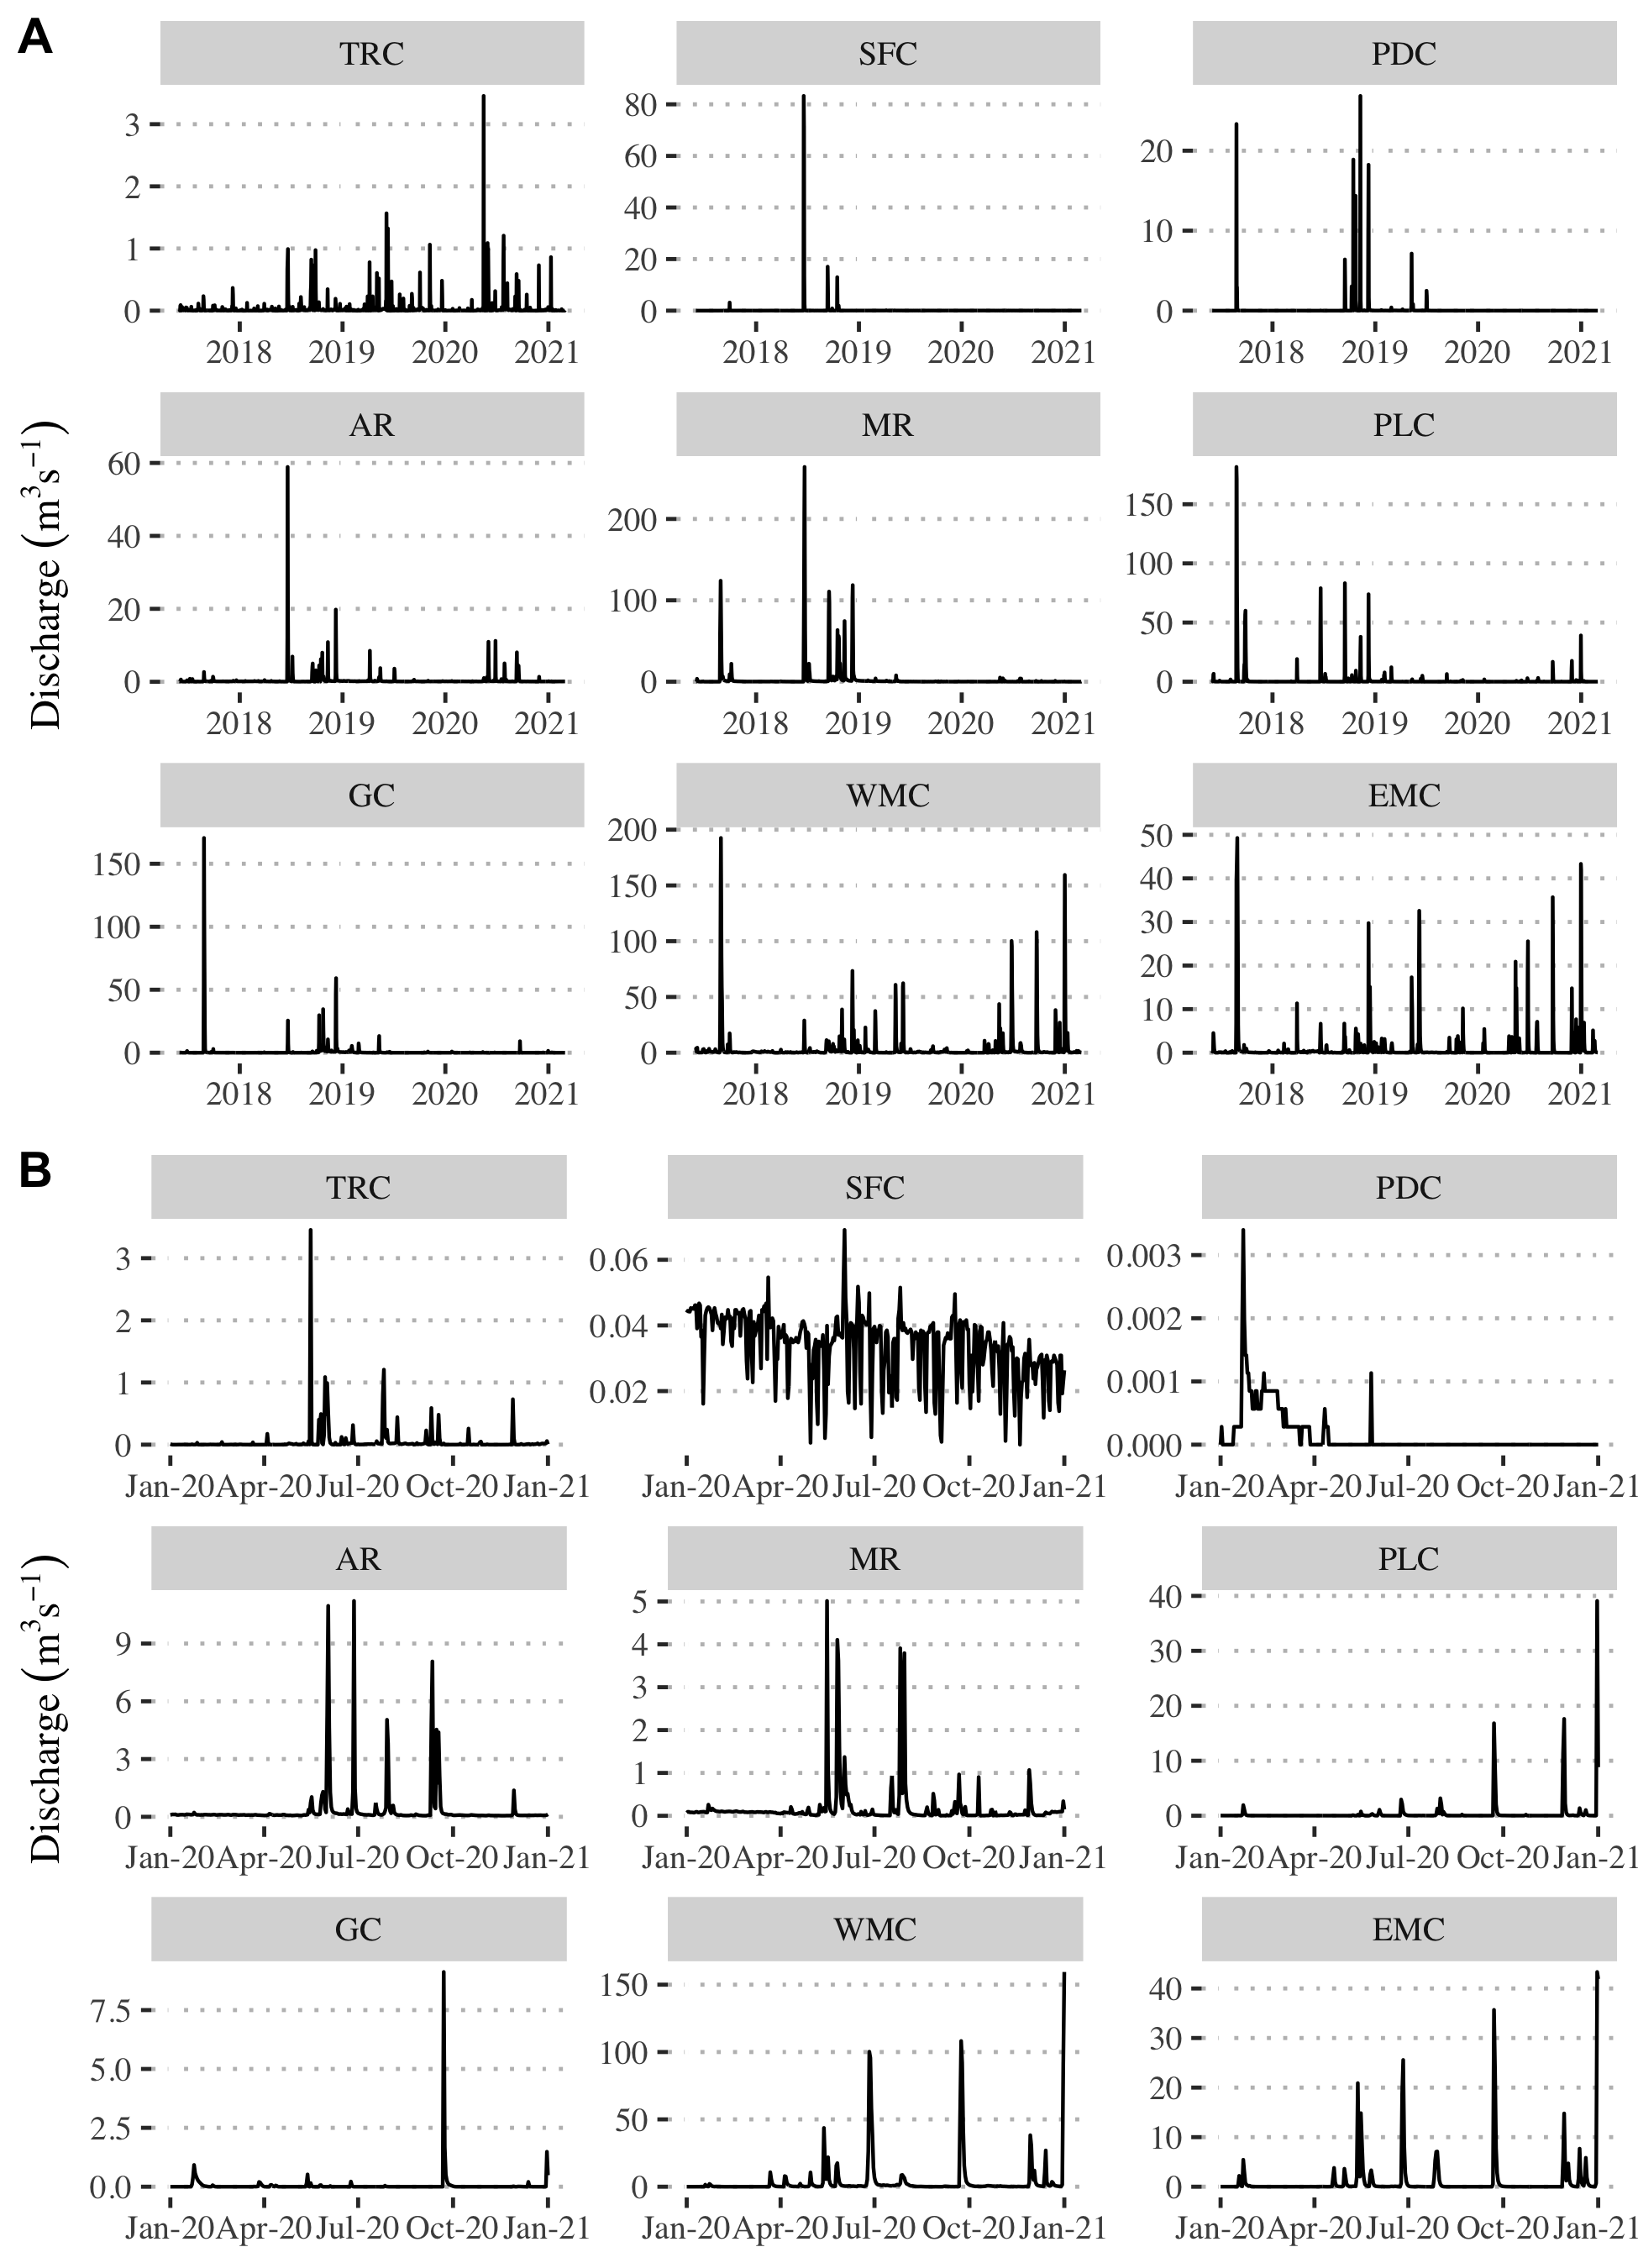
\includegraphics[scale = 0.21]{Figs/Q2020.png}
\caption[Site Discharge]{\textit{Site Discharge}. Sites are arranged arid to mesic left to right and top to bottom. Discharge appears to increase along the gradients, however they are punctuated by sharp increases due to rainfall. Note the different y-axis. Figure A is discharge over the study period, while figure B is 2020.}
\label{Fig:Q}
\end{center}
\end{figure}



\section{Principal Component Analysis and Structural Equation Model}

The PCA based on percentages of watershed land use categories identified two gradients in these sites. Land use-PC1, explaining 44.1\% of the variation, and was explained by wetlands, shrubs, and grasslands to cropland and developed land, while land use-PC2, explaining 29\% of the variation, ordered streams along a gradient of forest and pasture relative to other land uses  (Figure~\ref{Fig:PCA}). PC values were used as a proxy for watershed land use in the structural equation model to evaluate distal and proximal drivers of GPP and ER.

\begin{figure}[htb]
\begin{center}
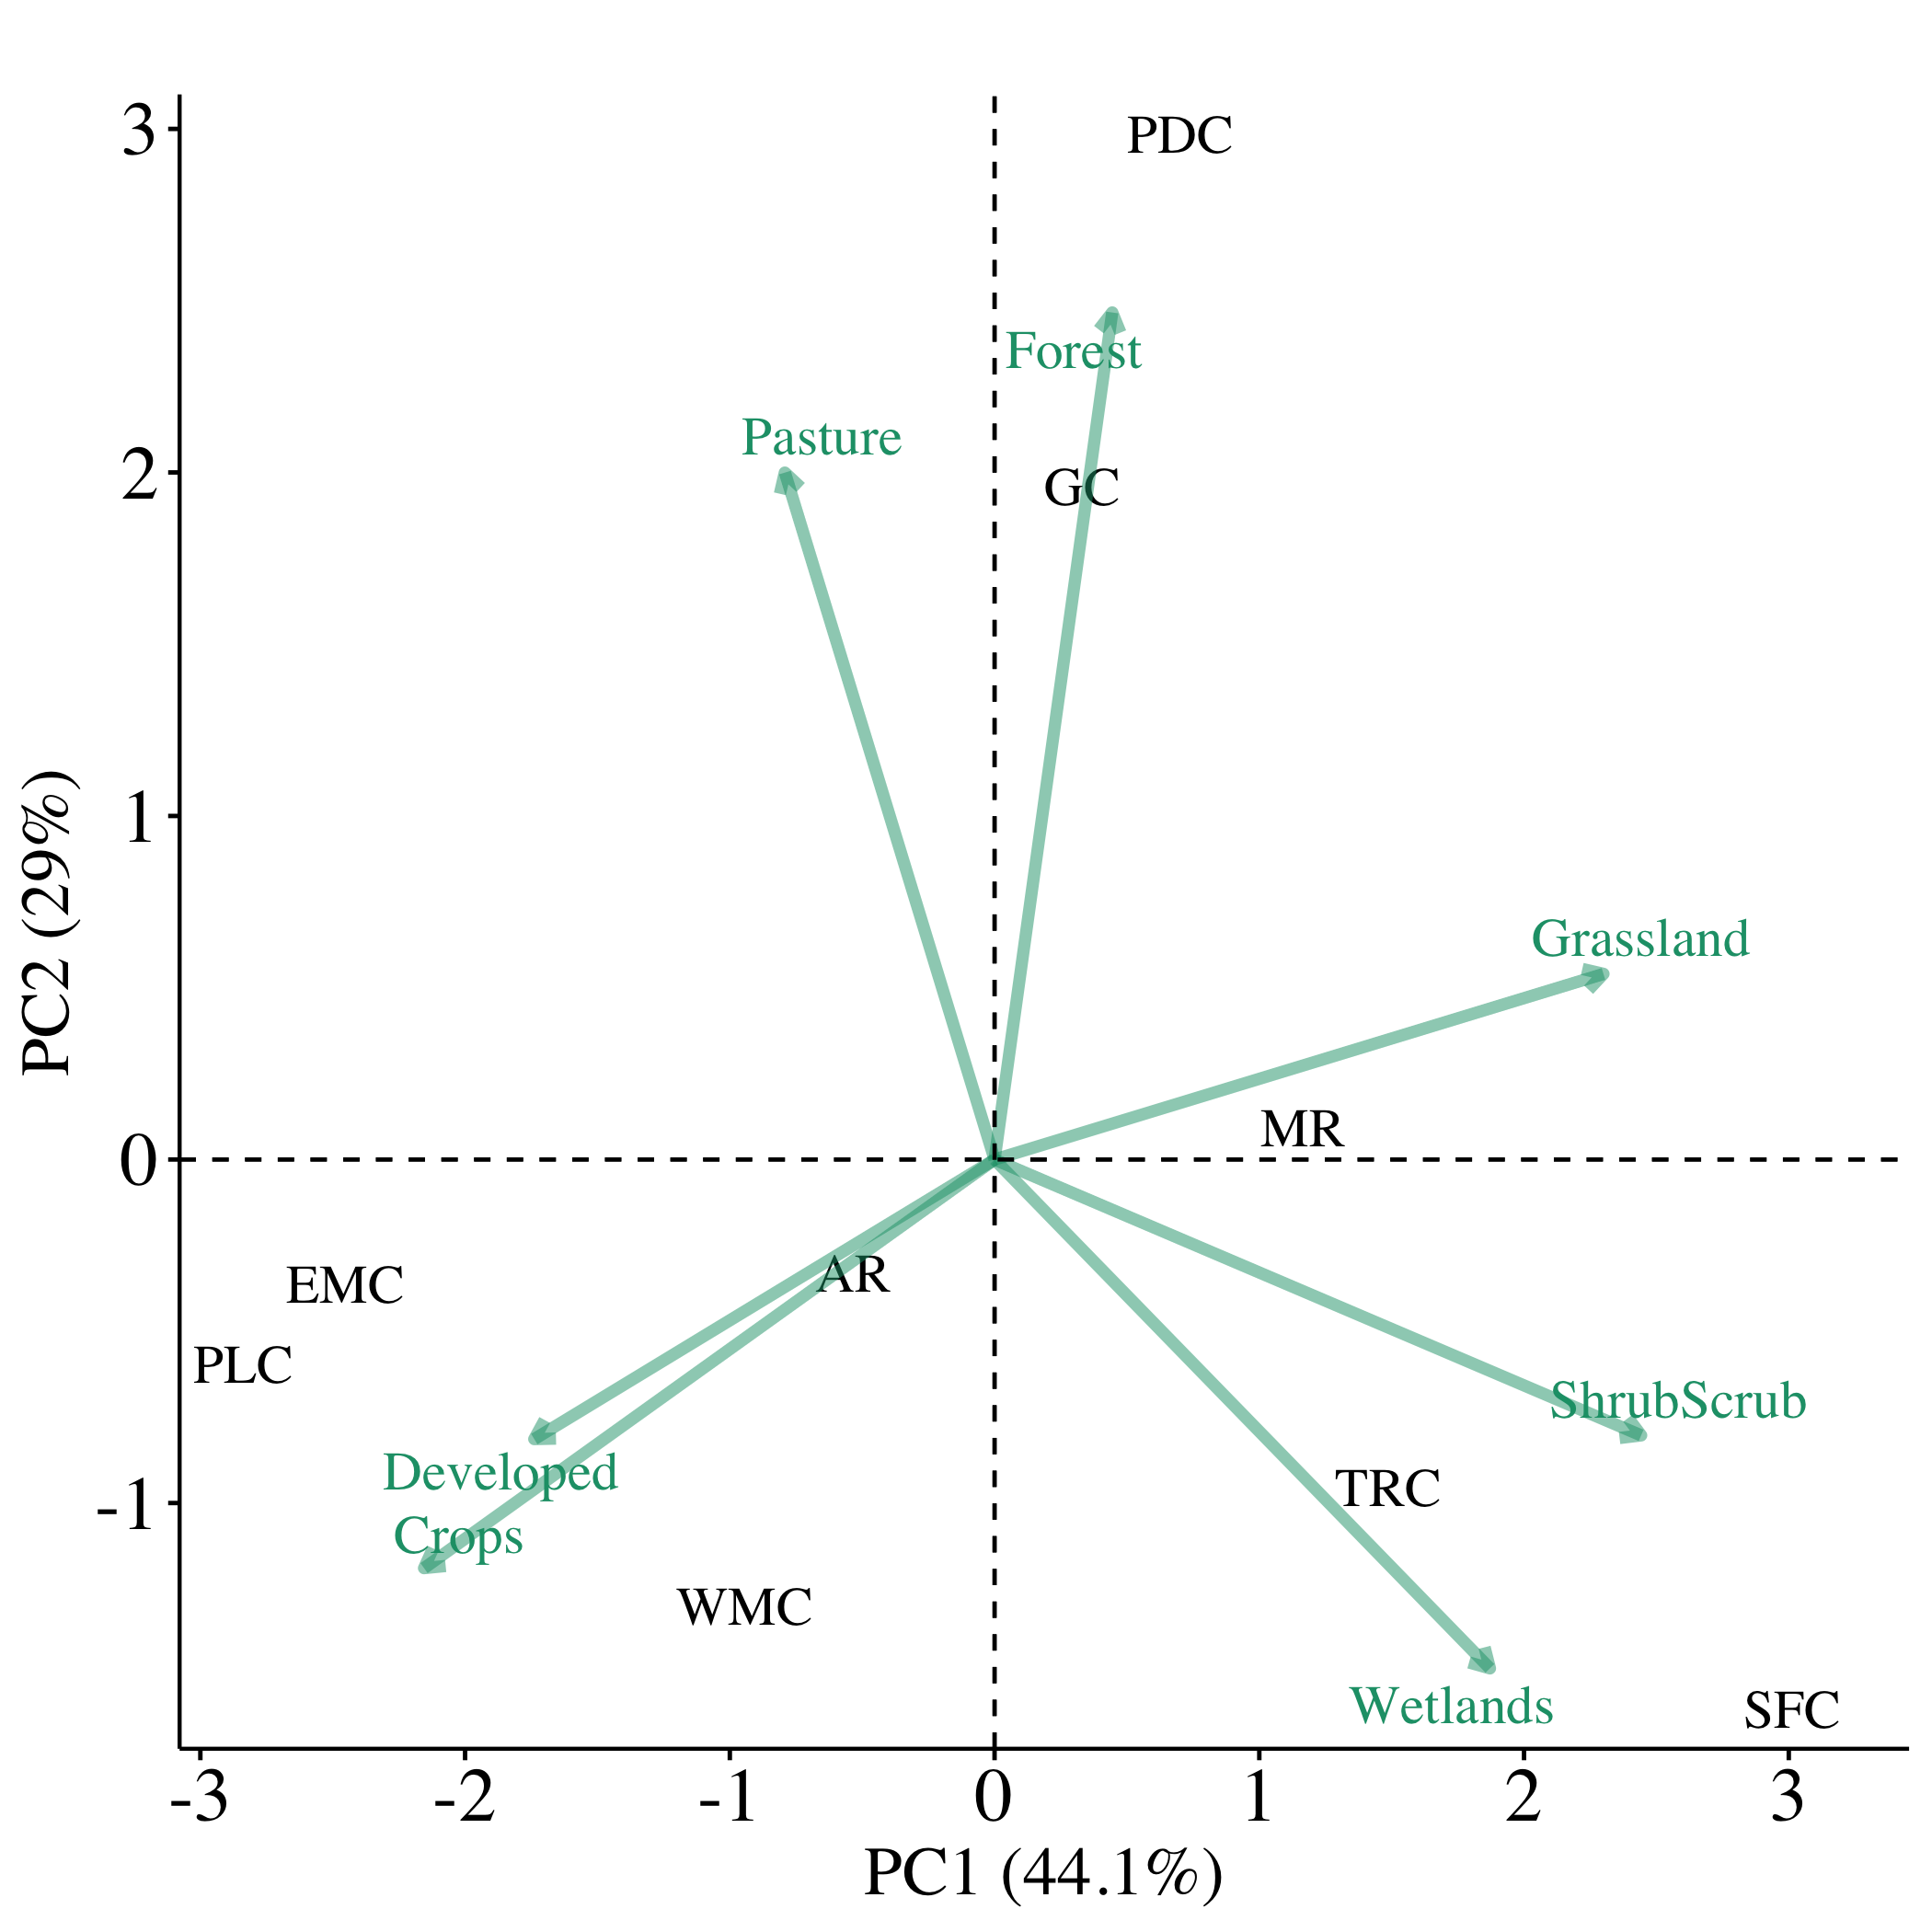
\includegraphics[scale=0.2]{Figs/PCA.png}
\caption[Principal Component Analysis]{\textit{Principal Component Analysis}. Principal component 1 ordered streams along a gradient of wetlands, shrubs, and grasslands to cropland and developed land, while principal component 2 grouped forest and pasture together.}
\label{Fig:PCA}
\end{center}
\end{figure}


I used a structural equation model to parse out the drivers of GPP and ER. I used the proximal drivers, average monthly precipitation, the presence of WWTP in the watershed, and land use PC1 and PC2 and distal drivers, discharge (CV), DOC, nitrate, and phosphate to explain the variability in monthly GPP and ER. I was unable to find a statistically significant model for the drivers of GPP and ER (Figure~\ref{Fig:SEMmetab}). However, when GPP and ER were removed from the model, there was a statistically significant model (Figure~\ref{Fig:SEMdrivers}). The results of the second SEM without GPP and ER indicated that land use PC1 and PC2 are strongly driving NO$_3$-N, PO$_4$-P, DOC, and turbidity, while monthly average precipitation is weakly driving NO$_3$-N and DOC.

\begin{landscape}
\begin{figure}[htb]
\begin{center}
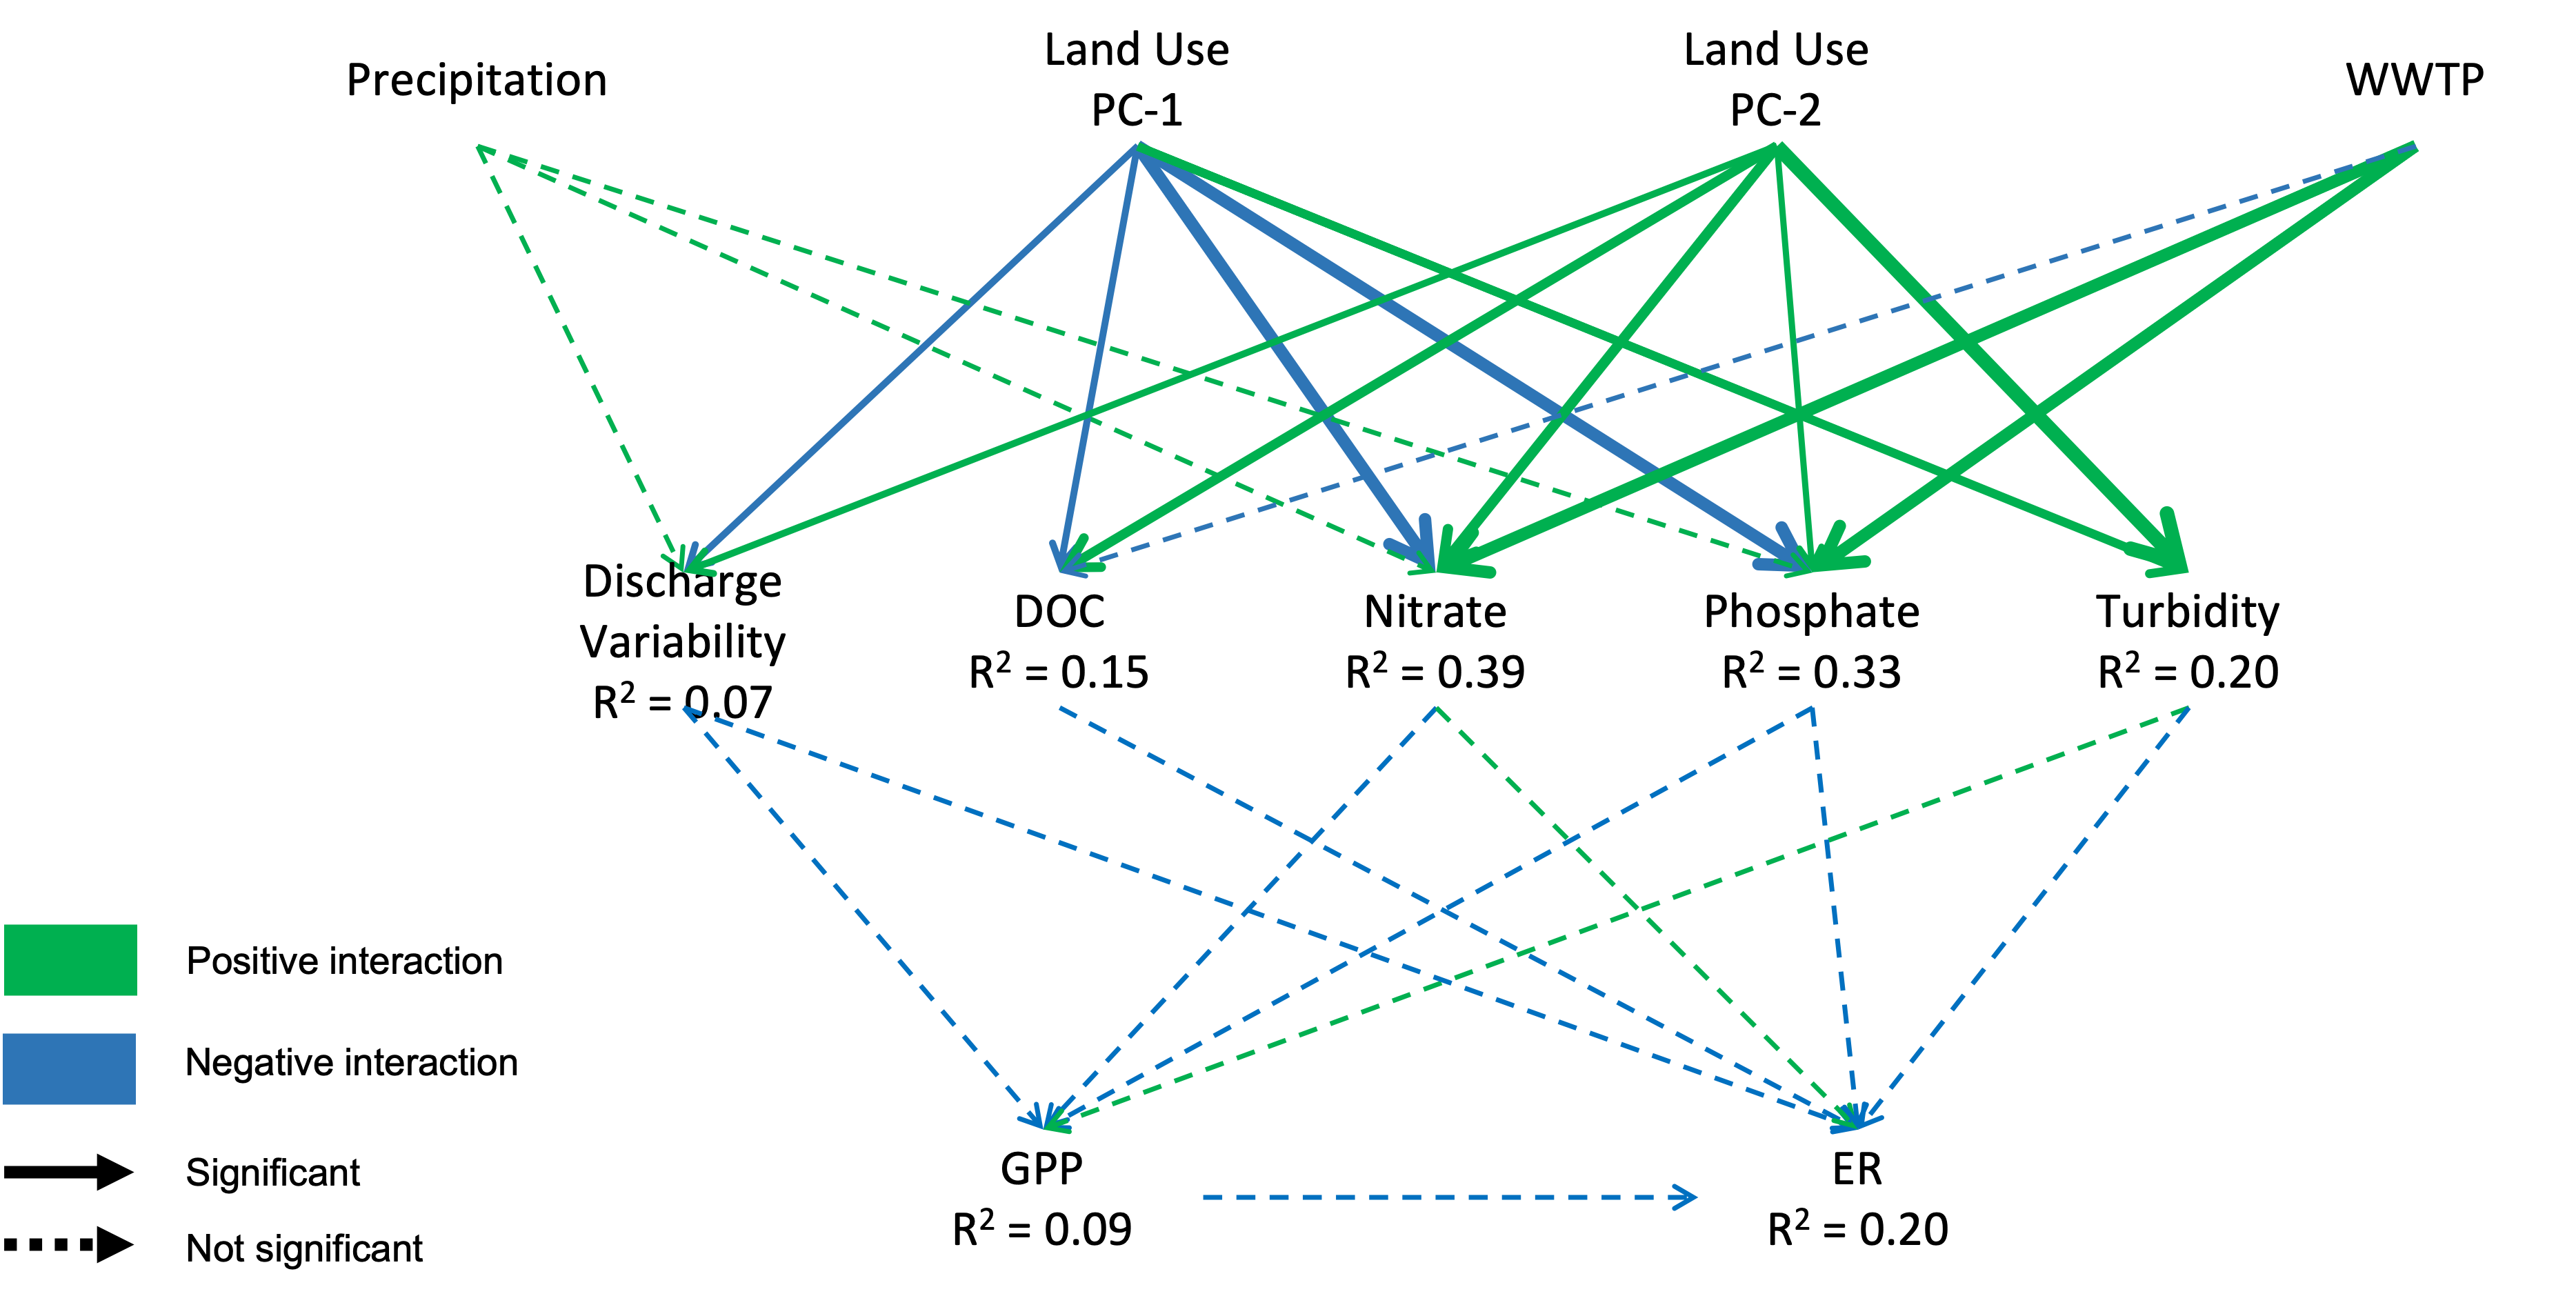
\includegraphics[scale=0.8]{Figs/SEMmetab.png}
\caption[SEM 1]{\textit{SEM 1}. The land use PCs (PC1 and PC2) and precipitation gradient had a strong impact on the proximal drivers (discharge, turbidity, DOC, nitrate, and phosphate), however, this interaction did not reach gross primary production or ecosystem respiration.}
\label{Fig:SEMmetab}
\end{center}
\end{figure}
\end{landscape}

\begin{landscape}
\begin{figure}[htb]
\begin{center}
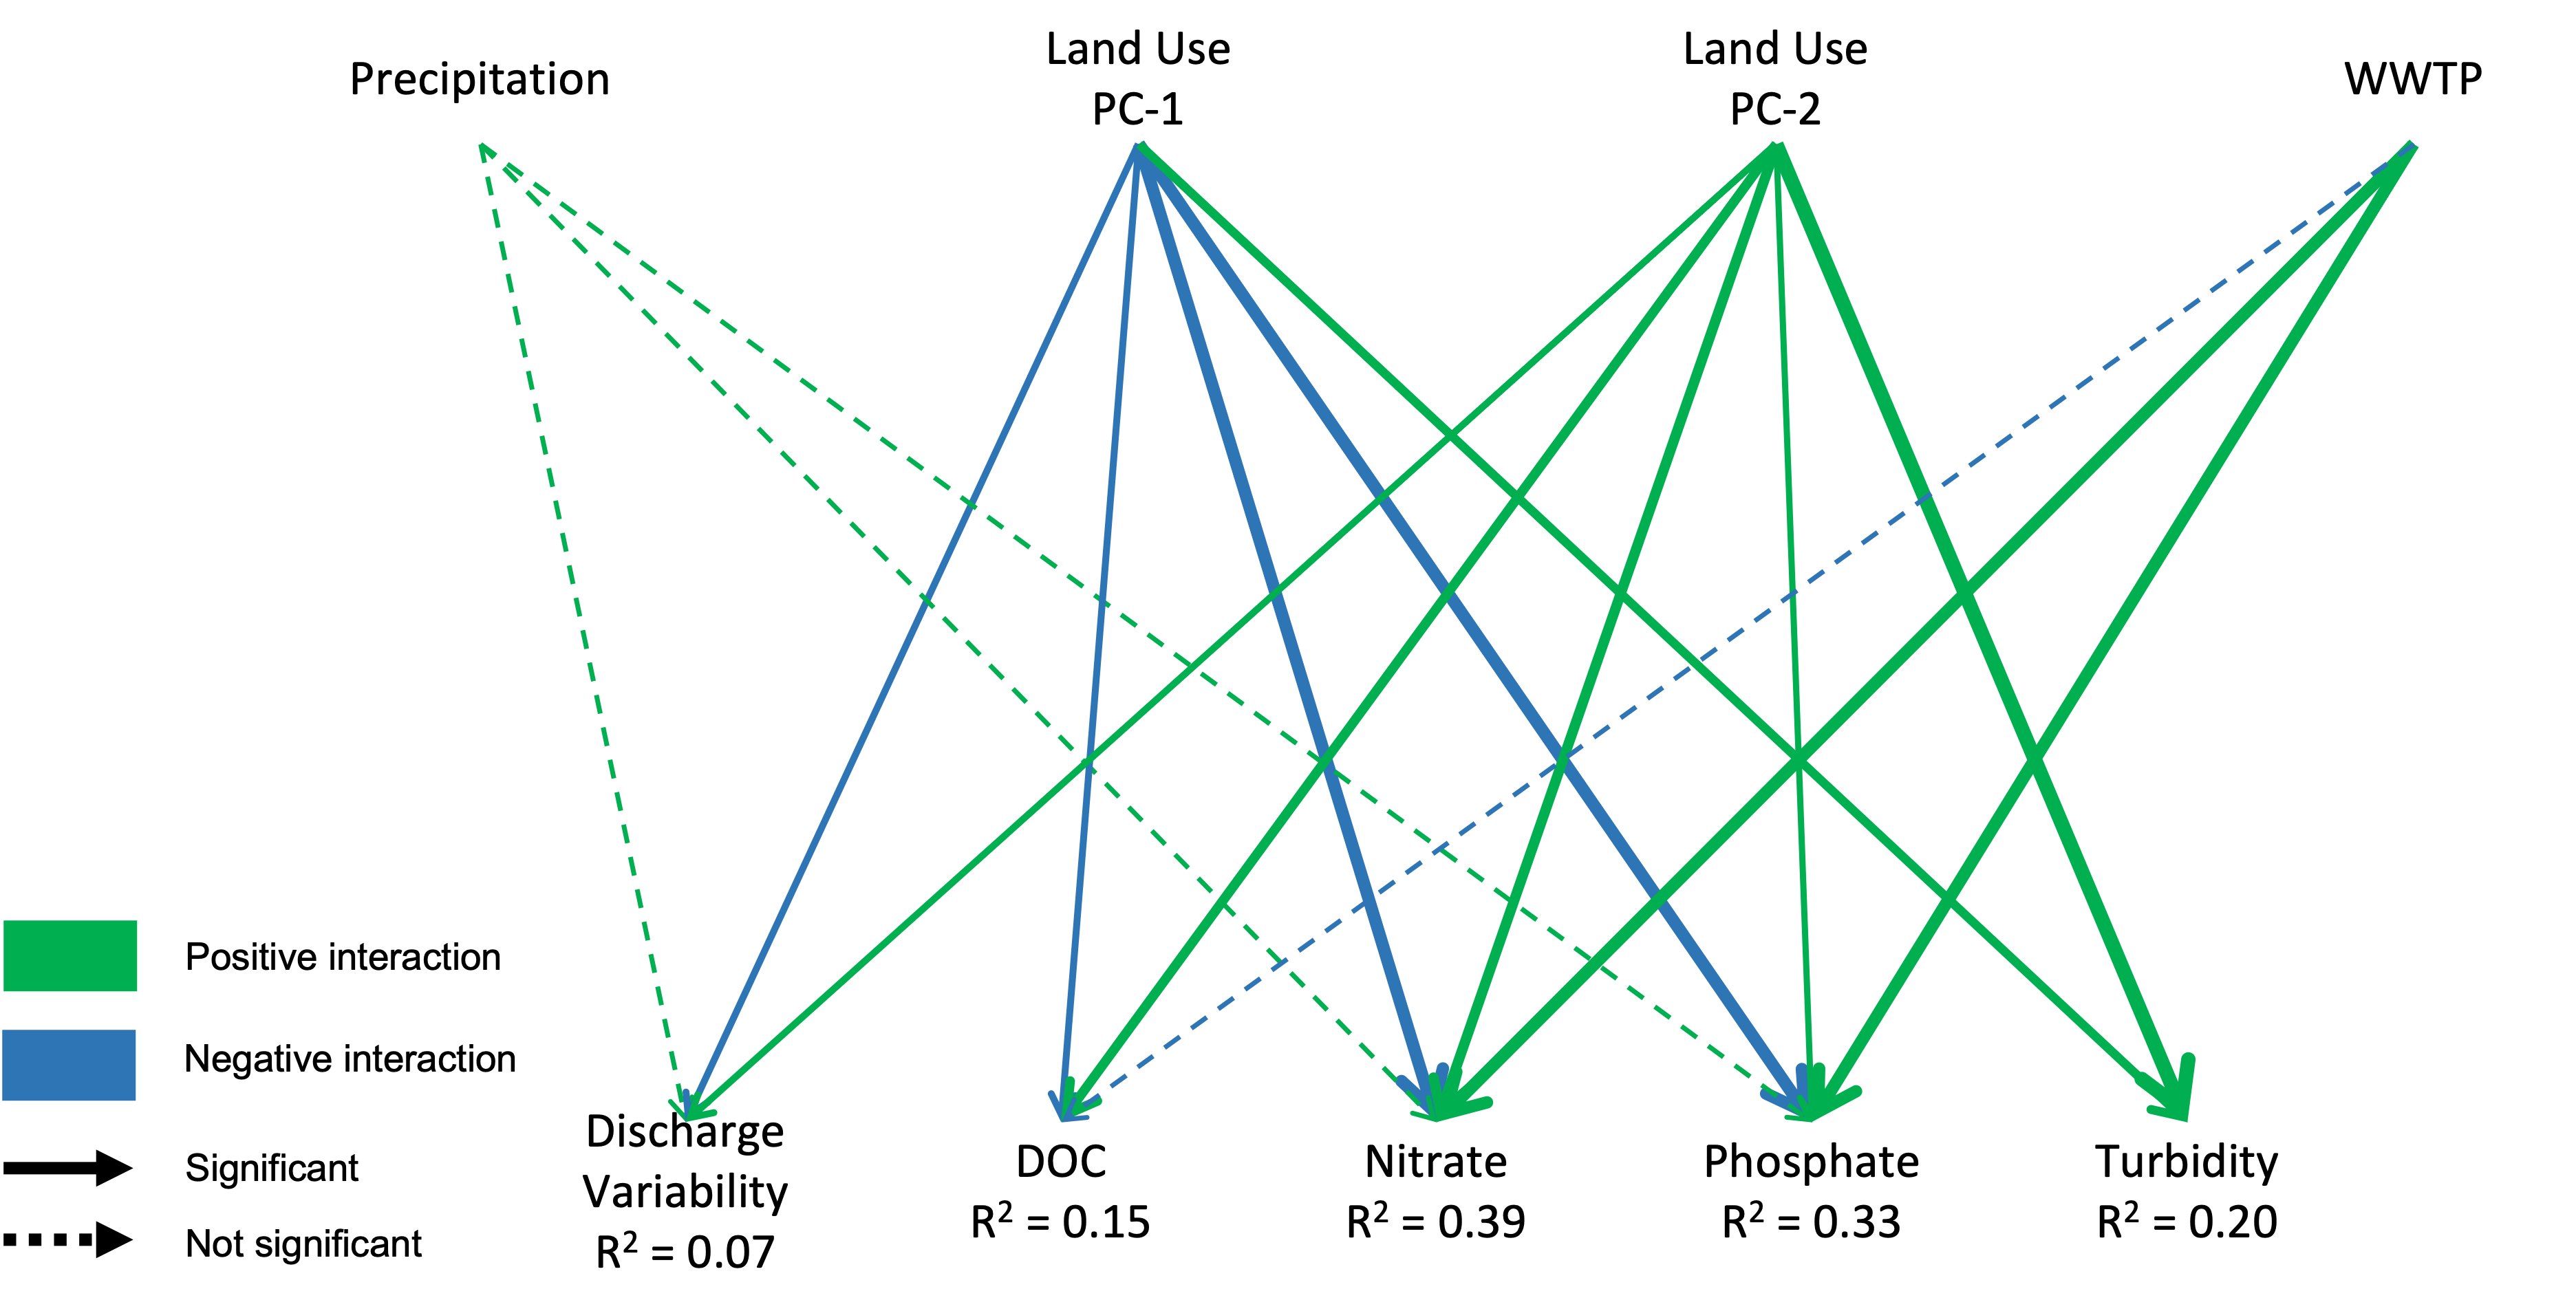
\includegraphics[scale=0.8]{Figs/SEMdrivers.png}
\caption[SEM 2]{\textit{SEM 2}. The land use PCs (PC1 and PC2) and precipitation gradient had a strong impact on proximal drivers (discharge, turbidity, DOC, nitrate, and phosphate).}
\label{Fig:SEMdrivers}
\end{center}
\end{figure}
\end{landscape}

\endinput

%-----------------------------------------------------------------------
% End of chap3.tex
%-----------------------------------------------------------------------
